\documentclass[twoside]{book}

% Packages required by doxygen
\usepackage{calc}
\usepackage{doxygen}
\usepackage{graphicx}
\usepackage[utf8]{inputenc}
\usepackage{makeidx}
\usepackage{multicol}
\usepackage{multirow}
\usepackage{textcomp}
\usepackage[table]{xcolor}

% NLS support packages
\usepackage[spanish]{babel}
% Font selection
\usepackage[T1]{fontenc}
\usepackage{mathptmx}
\usepackage[scaled=.90]{helvet}
\usepackage{courier}
\usepackage{amssymb}
\usepackage{sectsty}
\renewcommand{\familydefault}{\sfdefault}
\allsectionsfont{%
  \fontseries{bc}\selectfont%
  \color{darkgray}%
}
\renewcommand{\DoxyLabelFont}{%
  \fontseries{bc}\selectfont%
  \color{darkgray}%
}

% Page & text layout
\usepackage{geometry}
\geometry{%
  a4paper,%
  top=2.5cm,%
  bottom=2.5cm,%
  left=2.5cm,%
  right=2.5cm%
}
\tolerance=750
\hfuzz=15pt
\hbadness=750
\setlength{\emergencystretch}{15pt}
\setlength{\parindent}{0cm}
\setlength{\parskip}{0.2cm}
\makeatletter
\renewcommand{\paragraph}{%
  \@startsection{paragraph}{4}{0ex}{-1.0ex}{1.0ex}{%
    \normalfont\normalsize\bfseries\SS@parafont%
  }%
}
\renewcommand{\subparagraph}{%
  \@startsection{subparagraph}{5}{0ex}{-1.0ex}{1.0ex}{%
    \normalfont\normalsize\bfseries\SS@subparafont%
  }%
}
\makeatother

% Headers & footers
\usepackage{fancyhdr}
\pagestyle{fancyplain}
\fancyhead[LE]{\fancyplain{}{\bfseries\thepage}}
\fancyhead[CE]{\fancyplain{}{}}
\fancyhead[RE]{\fancyplain{}{\bfseries\leftmark}}
\fancyhead[LO]{\fancyplain{}{\bfseries\rightmark}}
\fancyhead[CO]{\fancyplain{}{}}
\fancyhead[RO]{\fancyplain{}{\bfseries\thepage}}
\fancyfoot[LE]{\fancyplain{}{}}
\fancyfoot[CE]{\fancyplain{}{}}
\fancyfoot[CO]{\fancyplain{}{}}
\fancyfoot[RO]{\fancyplain{}{}}
\renewcommand{\footrulewidth}{0.4pt}
\renewcommand{\chaptermark}[1]{%
  \markboth{#1}{}%
}
\renewcommand{\sectionmark}[1]{%
  \markright{\thesection\ #1}%
}

% Indices & bibliography
\usepackage{natbib}
\usepackage[titles]{tocloft}
\setcounter{tocdepth}{3}
\setcounter{secnumdepth}{5}
\makeindex

% Custom commands
\newcommand{\clearemptydoublepage}{%
  \newpage{\pagestyle{empty}\cleardoublepage}%
}


%===== C O N T E N T S =====

\begin{document}

% Titlepage & ToC
\pagenumbering{roman}
\begin{titlepage}
\vspace*{7cm}
\begin{center}%
{\Large S\-U\-D\-O\-K\-U }\\
\vspace*{1cm}
{\large Generado por Doxygen 1.8.4}\\
\vspace*{0.5cm}
\end{center}
\end{titlepage}
\clearemptydoublepage
\tableofcontents
\clearemptydoublepage
\pagenumbering{arabic}

%--- Begin generated contents ---
\chapter{Documentación de las clases}
\section{Referencia de la Clase Clock}
\label{class_clock}\index{Clock@{Clock}}


{\ttfamily \#include $<$clock.\-h$>$}



Diagrama de herencias de Clock
\nopagebreak
\begin{figure}[H]
\begin{center}
\leavevmode
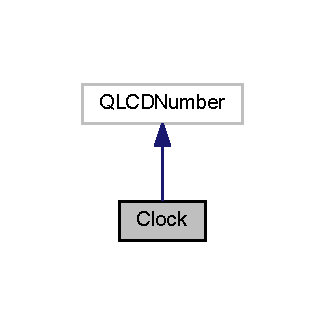
\includegraphics[width=156pt]{class_clock__inherit__graph}
\end{center}
\end{figure}


Diagrama de colaboración para Clock\-:
\nopagebreak
\begin{figure}[H]
\begin{center}
\leavevmode
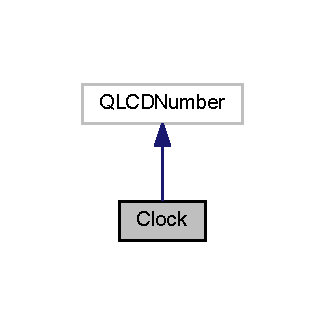
\includegraphics[width=156pt]{class_clock__coll__graph}
\end{center}
\end{figure}
\subsection*{Slots públicos}
\begin{DoxyCompactItemize}
\item 
void {\bf start\-Timer} ()
\item 
void {\bf stop\-Timer} ()
\item 
int {\bf get\-Time\-Score} ()
\end{DoxyCompactItemize}
\subsection*{Métodos públicos}
\begin{DoxyCompactItemize}
\item 
{\bf Clock} (Q\-Widget $\ast$parent=0)
\item 
{\bf $\sim$\-Clock} ()
\end{DoxyCompactItemize}
\subsection*{Atributos públicos}
\begin{DoxyCompactItemize}
\item 
int {\bf time\-Added}
\end{DoxyCompactItemize}
\subsection*{Slots privados}
\begin{DoxyCompactItemize}
\item 
void {\bf show\-Time} ()
\item 
void {\bf init\-Gui} ()
\end{DoxyCompactItemize}
\subsection*{Atributos privados}
\begin{DoxyCompactItemize}
\item 
Ui\-::\-Clock $\ast$ {\bf ui}
\item 
Q\-Time {\bf initial\-Time}
\item 
Q\-Timer $\ast$ {\bf timer}
\end{DoxyCompactItemize}


\subsection{Documentación del constructor y destructor}
\index{Clock@{Clock}!Clock@{Clock}}
\index{Clock@{Clock}!Clock@{Clock}}
\subsubsection[{Clock}]{\setlength{\rightskip}{0pt plus 5cm}Clock\-::\-Clock (
\begin{DoxyParamCaption}
\item[{Q\-Widget $\ast$}]{parent = {\ttfamily 0}}
\end{DoxyParamCaption}
)\hspace{0.3cm}{\ttfamily [explicit]}}\label{class_clock_adf2e47dbbb338cc358bc21a1ad934701}

\begin{DoxyCode}
6                             :
7     QLCDNumber(parent),
8     ui(\textcolor{keyword}{new} Ui::Clock)
9 \{
10     ui->setupUi(\textcolor{keyword}{this});
11     initGui();
12 \}
\end{DoxyCode}
\index{Clock@{Clock}!$\sim$\-Clock@{$\sim$\-Clock}}
\index{$\sim$\-Clock@{$\sim$\-Clock}!Clock@{Clock}}
\subsubsection[{$\sim$\-Clock}]{\setlength{\rightskip}{0pt plus 5cm}Clock\-::$\sim$\-Clock (
\begin{DoxyParamCaption}
{}
\end{DoxyParamCaption}
)}\label{class_clock_afc976ce68fa85e15cc06f9ed47bddb7c}

\begin{DoxyCode}
15 \{
16     \textcolor{keyword}{delete} timer;
17     \textcolor{keyword}{delete} ui;
18 \}
\end{DoxyCode}


\subsection{Documentación de las funciones miembro}
\index{Clock@{Clock}!get\-Time\-Score@{get\-Time\-Score}}
\index{get\-Time\-Score@{get\-Time\-Score}!Clock@{Clock}}
\subsubsection[{get\-Time\-Score}]{\setlength{\rightskip}{0pt plus 5cm}int Clock\-::get\-Time\-Score (
\begin{DoxyParamCaption}
{}
\end{DoxyParamCaption}
)\hspace{0.3cm}{\ttfamily [slot]}}\label{class_clock_aa3935c3a56349542716d9aecd79b7947}

\begin{DoxyCode}
54 \{
55     QTime time = QTime::currentTime();
56     time = time.addSecs(-initialTime.hour() * 3600 - initialTime.minute() * 60 - 
      initialTime.second());
57     \textcolor{keywordflow}{return} time.hour() * 3600 + time.minute() * 60 + time.second();
58 \}
\end{DoxyCode}
\index{Clock@{Clock}!init\-Gui@{init\-Gui}}
\index{init\-Gui@{init\-Gui}!Clock@{Clock}}
\subsubsection[{init\-Gui}]{\setlength{\rightskip}{0pt plus 5cm}void Clock\-::init\-Gui (
\begin{DoxyParamCaption}
{}
\end{DoxyParamCaption}
)\hspace{0.3cm}{\ttfamily [private]}, {\ttfamily [slot]}}\label{class_clock_af48d4217fe802dd730a62a12e997a607}

\begin{DoxyCode}
21 \{
22     setSegmentStyle(Filled);
23     setWindowTitle(tr(\textcolor{stringliteral}{"Timer"}));
24     resize(150, 60);
25 \}
\end{DoxyCode}
\index{Clock@{Clock}!show\-Time@{show\-Time}}
\index{show\-Time@{show\-Time}!Clock@{Clock}}
\subsubsection[{show\-Time}]{\setlength{\rightskip}{0pt plus 5cm}void Clock\-::show\-Time (
\begin{DoxyParamCaption}
{}
\end{DoxyParamCaption}
)\hspace{0.3cm}{\ttfamily [private]}, {\ttfamily [slot]}}\label{class_clock_adb348ce7f498c58896a67e4f87b9a165}

\begin{DoxyCode}
28 \{
29     QTime time = QTime::currentTime();
30     time = time.addSecs(-initialTime.hour() * 3600 - initialTime.minute() * 60 - 
      initialTime.second());
31     time = time.addSecs(timeAdded);
32     QString text = time.toString(\textcolor{stringliteral}{"hh:mm:ss"});
33 
34     display(text);
35 \}
\end{DoxyCode}
\index{Clock@{Clock}!start\-Timer@{start\-Timer}}
\index{start\-Timer@{start\-Timer}!Clock@{Clock}}
\subsubsection[{start\-Timer}]{\setlength{\rightskip}{0pt plus 5cm}void Clock\-::start\-Timer (
\begin{DoxyParamCaption}
{}
\end{DoxyParamCaption}
)\hspace{0.3cm}{\ttfamily [slot]}}\label{class_clock_a4c236255a43ef536932608ae3bc71033}

\begin{DoxyCode}
38 \{
39     timer = \textcolor{keyword}{new} QTimer(\textcolor{keyword}{this});
40     connect(timer, SIGNAL(timeout()), \textcolor{keyword}{this}, SLOT(showTime()));
41     timer->start(1000);
42 
43     initialTime = QTime::currentTime();
44     display(\textcolor{stringliteral}{"00:00"});
45     showTime();
46 \}
\end{DoxyCode}
\index{Clock@{Clock}!stop\-Timer@{stop\-Timer}}
\index{stop\-Timer@{stop\-Timer}!Clock@{Clock}}
\subsubsection[{stop\-Timer}]{\setlength{\rightskip}{0pt plus 5cm}void Clock\-::stop\-Timer (
\begin{DoxyParamCaption}
{}
\end{DoxyParamCaption}
)\hspace{0.3cm}{\ttfamily [slot]}}\label{class_clock_ad687c99536ba2b5578b77b208d7e3fdf}

\begin{DoxyCode}
49 \{
50     timer->stop();
51 \}
\end{DoxyCode}


\subsection{Documentación de los datos miembro}
\index{Clock@{Clock}!initial\-Time@{initial\-Time}}
\index{initial\-Time@{initial\-Time}!Clock@{Clock}}
\subsubsection[{initial\-Time}]{\setlength{\rightskip}{0pt plus 5cm}Q\-Time Clock\-::initial\-Time\hspace{0.3cm}{\ttfamily [private]}}\label{class_clock_ad06c7d67265fe4b6909be8e95e669490}
\index{Clock@{Clock}!time\-Added@{time\-Added}}
\index{time\-Added@{time\-Added}!Clock@{Clock}}
\subsubsection[{time\-Added}]{\setlength{\rightskip}{0pt plus 5cm}int Clock\-::time\-Added}\label{class_clock_ae2a6285de90ddc3a034d4fd9982e8c24}
\index{Clock@{Clock}!timer@{timer}}
\index{timer@{timer}!Clock@{Clock}}
\subsubsection[{timer}]{\setlength{\rightskip}{0pt plus 5cm}Q\-Timer$\ast$ Clock\-::timer\hspace{0.3cm}{\ttfamily [private]}}\label{class_clock_ab51e4108c5a6a16e851cad646e77d9ba}
\index{Clock@{Clock}!ui@{ui}}
\index{ui@{ui}!Clock@{Clock}}
\subsubsection[{ui}]{\setlength{\rightskip}{0pt plus 5cm}Ui\-::\-Clock$\ast$ Clock\-::ui\hspace{0.3cm}{\ttfamily [private]}}\label{class_clock_a60b333971122a727784de3d380642a4d}


La documentación para esta clase fue generada a partir de los siguientes ficheros\-:\begin{DoxyCompactItemize}
\item 
I\-:/\-Sudoku-\/master/\-Sudoku/\-Functional Version/{\bf clock.\-h}\item 
I\-:/\-Sudoku-\/master/\-Sudoku/\-Functional Version/{\bf clock.\-cpp}\end{DoxyCompactItemize}

\section{Referencia de la Clase Q\-Push\-Button\-Grid}
\label{class_q_push_button_grid}\index{Q\-Push\-Button\-Grid@{Q\-Push\-Button\-Grid}}


{\ttfamily \#include $<$qpushbuttongrid.\-h$>$}



Diagrama de herencias de Q\-Push\-Button\-Grid
\nopagebreak
\begin{figure}[H]
\begin{center}
\leavevmode
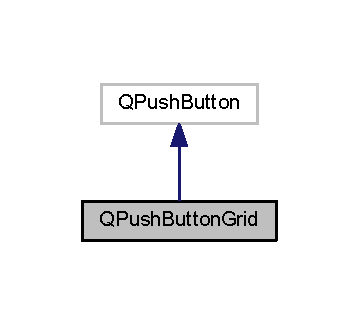
\includegraphics[width=172pt]{class_q_push_button_grid__inherit__graph}
\end{center}
\end{figure}


Diagrama de colaboración para Q\-Push\-Button\-Grid\-:
\nopagebreak
\begin{figure}[H]
\begin{center}
\leavevmode
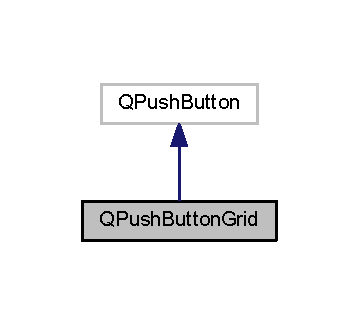
\includegraphics[width=172pt]{class_q_push_button_grid__coll__graph}
\end{center}
\end{figure}
\subsection*{Métodos públicos}
\begin{DoxyCompactItemize}
\item 
{\bf Q\-Push\-Button\-Grid} (Q\-Push\-Button $\ast$parent=0)
\item 
{\bf $\sim$\-Q\-Push\-Button\-Grid} ()
\end{DoxyCompactItemize}
\subsection*{Atributos públicos}
\begin{DoxyCompactItemize}
\item 
int {\bf row}
\item 
int {\bf column}
\item 
int {\bf real\-Number}
\item 
int {\bf assigned\-Number}
\item 
int {\bf color}
\item 
bool {\bf is\-Constant}
\end{DoxyCompactItemize}
\subsection*{Atributos privados}
\begin{DoxyCompactItemize}
\item 
Ui\-::\-Q\-Push\-Button\-Grid $\ast$ {\bf ui}
\end{DoxyCompactItemize}


\subsection{Documentación del constructor y destructor}
\index{Q\-Push\-Button\-Grid@{Q\-Push\-Button\-Grid}!Q\-Push\-Button\-Grid@{Q\-Push\-Button\-Grid}}
\index{Q\-Push\-Button\-Grid@{Q\-Push\-Button\-Grid}!QPushButtonGrid@{Q\-Push\-Button\-Grid}}
\subsubsection[{Q\-Push\-Button\-Grid}]{\setlength{\rightskip}{0pt plus 5cm}Q\-Push\-Button\-Grid\-::\-Q\-Push\-Button\-Grid (
\begin{DoxyParamCaption}
\item[{Q\-Push\-Button $\ast$}]{parent = {\ttfamily 0}}
\end{DoxyParamCaption}
)\hspace{0.3cm}{\ttfamily [explicit]}}\label{class_q_push_button_grid_a44014c8f870815c07dd1ffa8def17f40}

\begin{DoxyCode}
4                                                     :
5     QPushButton(parent),
6     ui(\textcolor{keyword}{new} Ui::QPushButtonGrid)
7 \{
8     ui->setupUi(\textcolor{keyword}{this});
9 \}
\end{DoxyCode}
\index{Q\-Push\-Button\-Grid@{Q\-Push\-Button\-Grid}!$\sim$\-Q\-Push\-Button\-Grid@{$\sim$\-Q\-Push\-Button\-Grid}}
\index{$\sim$\-Q\-Push\-Button\-Grid@{$\sim$\-Q\-Push\-Button\-Grid}!QPushButtonGrid@{Q\-Push\-Button\-Grid}}
\subsubsection[{$\sim$\-Q\-Push\-Button\-Grid}]{\setlength{\rightskip}{0pt plus 5cm}Q\-Push\-Button\-Grid\-::$\sim$\-Q\-Push\-Button\-Grid (
\begin{DoxyParamCaption}
{}
\end{DoxyParamCaption}
)}\label{class_q_push_button_grid_a34d347faea34c64fe1dd3018254dea86}

\begin{DoxyCode}
12 \{
13     \textcolor{keyword}{delete} ui;
14 \}
\end{DoxyCode}


\subsection{Documentación de los datos miembro}
\index{Q\-Push\-Button\-Grid@{Q\-Push\-Button\-Grid}!assigned\-Number@{assigned\-Number}}
\index{assigned\-Number@{assigned\-Number}!QPushButtonGrid@{Q\-Push\-Button\-Grid}}
\subsubsection[{assigned\-Number}]{\setlength{\rightskip}{0pt plus 5cm}int Q\-Push\-Button\-Grid\-::assigned\-Number}\label{class_q_push_button_grid_a17927930ad86813a22795fd246de1c7c}
\index{Q\-Push\-Button\-Grid@{Q\-Push\-Button\-Grid}!color@{color}}
\index{color@{color}!QPushButtonGrid@{Q\-Push\-Button\-Grid}}
\subsubsection[{color}]{\setlength{\rightskip}{0pt plus 5cm}int Q\-Push\-Button\-Grid\-::color}\label{class_q_push_button_grid_ab8ed3340d216292a440b865dd8784bc8}
\index{Q\-Push\-Button\-Grid@{Q\-Push\-Button\-Grid}!column@{column}}
\index{column@{column}!QPushButtonGrid@{Q\-Push\-Button\-Grid}}
\subsubsection[{column}]{\setlength{\rightskip}{0pt plus 5cm}int Q\-Push\-Button\-Grid\-::column}\label{class_q_push_button_grid_a48a98134fc3fd27f119310ba06702e99}
\index{Q\-Push\-Button\-Grid@{Q\-Push\-Button\-Grid}!is\-Constant@{is\-Constant}}
\index{is\-Constant@{is\-Constant}!QPushButtonGrid@{Q\-Push\-Button\-Grid}}
\subsubsection[{is\-Constant}]{\setlength{\rightskip}{0pt plus 5cm}bool Q\-Push\-Button\-Grid\-::is\-Constant}\label{class_q_push_button_grid_aec9a55983edc0ecea663a4445b1fa0cb}
\index{Q\-Push\-Button\-Grid@{Q\-Push\-Button\-Grid}!real\-Number@{real\-Number}}
\index{real\-Number@{real\-Number}!QPushButtonGrid@{Q\-Push\-Button\-Grid}}
\subsubsection[{real\-Number}]{\setlength{\rightskip}{0pt plus 5cm}int Q\-Push\-Button\-Grid\-::real\-Number}\label{class_q_push_button_grid_a659917a93c5ea84f8d6815a2380b687e}
\index{Q\-Push\-Button\-Grid@{Q\-Push\-Button\-Grid}!row@{row}}
\index{row@{row}!QPushButtonGrid@{Q\-Push\-Button\-Grid}}
\subsubsection[{row}]{\setlength{\rightskip}{0pt plus 5cm}int Q\-Push\-Button\-Grid\-::row}\label{class_q_push_button_grid_ad30c980cad65086f41840f69b5fb1e57}
\index{Q\-Push\-Button\-Grid@{Q\-Push\-Button\-Grid}!ui@{ui}}
\index{ui@{ui}!QPushButtonGrid@{Q\-Push\-Button\-Grid}}
\subsubsection[{ui}]{\setlength{\rightskip}{0pt plus 5cm}Ui\-::\-Q\-Push\-Button\-Grid$\ast$ Q\-Push\-Button\-Grid\-::ui\hspace{0.3cm}{\ttfamily [private]}}\label{class_q_push_button_grid_a73f52fa22fa7c71fa8401ad3890a9b86}


La documentación para esta clase fue generada a partir de los siguientes ficheros\-:\begin{DoxyCompactItemize}
\item 
I\-:/\-Sudoku-\/master/\-Sudoku/\-Functional Version/{\bf qpushbuttongrid.\-h}\item 
I\-:/\-Sudoku-\/master/\-Sudoku/\-Functional Version/{\bf qpushbuttongrid.\-cpp}\end{DoxyCompactItemize}

\section{Referencia de la Clase Sudoku}
\label{class_sudoku}\index{Sudoku@{Sudoku}}


{\ttfamily \#include $<$sudoku.\-h$>$}



Diagrama de herencias de Sudoku
\nopagebreak
\begin{figure}[H]
\begin{center}
\leavevmode
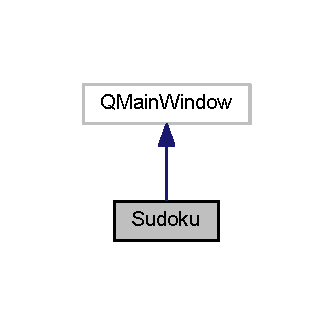
\includegraphics[width=160pt]{class_sudoku__inherit__graph}
\end{center}
\end{figure}


Diagrama de colaboración para Sudoku\-:
\nopagebreak
\begin{figure}[H]
\begin{center}
\leavevmode
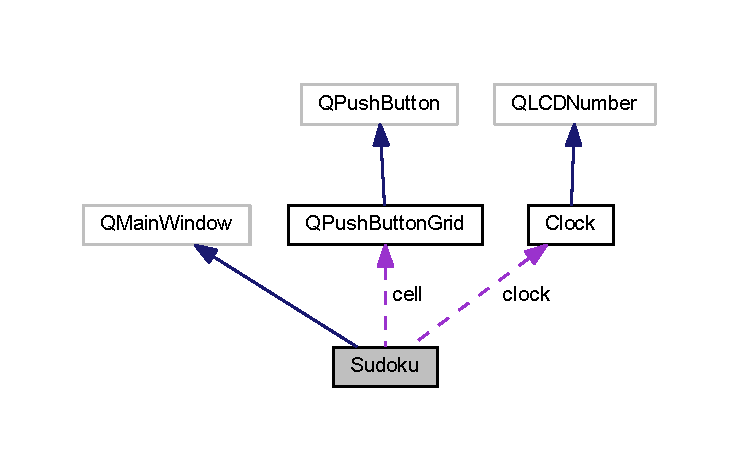
\includegraphics[width=350pt]{class_sudoku__coll__graph}
\end{center}
\end{figure}
\subsection*{Métodos públicos}
\begin{DoxyCompactItemize}
\item 
{\bf Sudoku} (Q\-Widget $\ast$parent=0)
\item 
{\bf $\sim$\-Sudoku} ()
\end{DoxyCompactItemize}
\subsection*{Slots privados}
\begin{DoxyCompactItemize}
\item 
void {\bf init\-Gui} ()
\item 
bool {\bf validate\-Cell\-At\-Point\-With\-Number} (int row, int column, int value, int counter)
\item 
bool {\bf number\-Assigner} (int counter, int row, int column, int value)
\item 
void {\bf sudoku\-Generator} (int row)
\item 
bool {\bf sudoku\-Blank\-Checker} ()
\item 
void {\bf sudoku\-Error\-Wiper} ()
\item 
bool {\bf is\-Sudoku\-Complete} ()
\begin{DoxyCompactList}\small\item\em Funcion Booleana \doxyref{Sudoku}{p.}{class_sudoku} Completo. \end{DoxyCompactList}\item 
void {\bf number\-\_\-clicked} ()
\item 
void {\bf cell\-\_\-clicked} ()
\item 
void {\bf on\-\_\-null\-Button\-\_\-clicked} ()
\item 
void {\bf validate\-Cell} ()
\item 
void {\bf on\-\_\-action\-New\-\_\-triggered} ()
\item 
void {\bf on\-\_\-action\-Open\-\_\-triggered} ()
\item 
void {\bf on\-\_\-action\-Save\-\_\-triggered} ()
\item 
void {\bf on\-\_\-action\-Close\-\_\-triggered} ()
\item 
void {\bf on\-\_\-action\-Quit\-\_\-triggered} ()
\item 
void {\bf validate\-Window} ()
\item 
void {\bf invalidate\-Window} ()
\item 
void {\bf on\-\_\-push\-Button\-\_\-clicked} ()
\item 
void {\bf on\-\_\-normal\-Button\-\_\-clicked} ()
\begin{DoxyCompactList}\small\item\em Game Mode Normal (Modo de Juego) \end{DoxyCompactList}\item 
void {\bf on\-\_\-hint\-Button\-\_\-clicked} ()
\begin{DoxyCompactList}\small\item\em Game Mode Hint (Modo de Juego Hint) \end{DoxyCompactList}\item 
void {\bf on\-\_\-clue\-Button\-\_\-clicked} ()
\begin{DoxyCompactList}\small\item\em Game Mode Clue(\-Modo de Juego) \end{DoxyCompactList}\item 
void {\bf on\-\_\-action\-Easy\-\_\-triggered} ()
\begin{DoxyCompactList}\small\item\em Nivel F\-A\-C\-I\-L. \end{DoxyCompactList}\item 
void {\bf on\-\_\-action\-Medium\-\_\-triggered} ()
\begin{DoxyCompactList}\small\item\em Nivel D\-I\-F\-I\-C\-I\-L. \end{DoxyCompactList}\item 
void {\bf on\-\_\-action\-Hard\-\_\-triggered} ()
\begin{DoxyCompactList}\small\item\em Nivel D\-I\-F\-I\-C\-I\-L. \end{DoxyCompactList}\end{DoxyCompactItemize}
\subsection*{Atributos privados}
\begin{DoxyCompactItemize}
\item 
Ui\-::\-Sudoku $\ast$ {\bf ui}
\item 
{\bf Q\-Push\-Button\-Grid} $\ast$ {\bf cell} [9][9]
\item 
Q\-Push\-Button $\ast$ {\bf number} [9]
\item 
Q\-String {\bf crypt}
\item 
{\bf Clock} $\ast$ {\bf clock}
\item 
int {\bf coor\-X}
\item 
int {\bf coor\-Y}
\item 
bool {\bf is\-Cell\-Selected}
\end{DoxyCompactItemize}


\subsection{Documentación del constructor y destructor}
\index{Sudoku@{Sudoku}!Sudoku@{Sudoku}}
\index{Sudoku@{Sudoku}!Sudoku@{Sudoku}}
\subsubsection[{Sudoku}]{\setlength{\rightskip}{0pt plus 5cm}Sudoku\-::\-Sudoku (
\begin{DoxyParamCaption}
\item[{Q\-Widget $\ast$}]{parent = {\ttfamily 0}}
\end{DoxyParamCaption}
)\hspace{0.3cm}{\ttfamily [explicit]}}\label{class_sudoku_a668fb7917f321f44537700627aff6f6f}

\begin{DoxyCode}
19                               :
20     QMainWindow(parent),
21     ui(\textcolor{keyword}{new} Ui::Sudoku)
22 \{
23     srand((\textcolor{keywordtype}{unsigned})time(NULL));
24     ui->setupUi(\textcolor{keyword}{this});
25     initGui();
26 \}
\end{DoxyCode}
\index{Sudoku@{Sudoku}!$\sim$\-Sudoku@{$\sim$\-Sudoku}}
\index{$\sim$\-Sudoku@{$\sim$\-Sudoku}!Sudoku@{Sudoku}}
\subsubsection[{$\sim$\-Sudoku}]{\setlength{\rightskip}{0pt plus 5cm}Sudoku\-::$\sim$\-Sudoku (
\begin{DoxyParamCaption}
{}
\end{DoxyParamCaption}
)}\label{class_sudoku_a9c949b824fa3d98d3515dbecb8cf413e}

\begin{DoxyCode}
29 \{
30     \textcolor{keyword}{delete} ui;
31     \textcolor{keywordflow}{for} (\textcolor{keywordtype}{int} i = 0; i < 9; i++)
32     \{
33         \textcolor{keywordflow}{for}(\textcolor{keywordtype}{int} j = 0; j < 9; j++)
34         \{
35             \textcolor{keyword}{delete} cell[i][j];
36         \}
37     \}
38     \textcolor{keywordflow}{for} (\textcolor{keywordtype}{int} i = 0; i < 9; i++)
39     \{
40         \textcolor{keyword}{delete} number[i];
41 
42     \}
43     \textcolor{keyword}{delete} clock;
44 \}
\end{DoxyCode}


\subsection{Documentación de las funciones miembro}
\index{Sudoku@{Sudoku}!cell\-\_\-clicked@{cell\-\_\-clicked}}
\index{cell\-\_\-clicked@{cell\-\_\-clicked}!Sudoku@{Sudoku}}
\subsubsection[{cell\-\_\-clicked}]{\setlength{\rightskip}{0pt plus 5cm}void Sudoku\-::cell\-\_\-clicked (
\begin{DoxyParamCaption}
{}
\end{DoxyParamCaption}
)\hspace{0.3cm}{\ttfamily [private]}, {\ttfamily [slot]}}\label{class_sudoku_a660ca7cc295d016f2a4d707367acc9d5}

\begin{DoxyCode}
364 \{
365     \textcolor{keywordflow}{if} (!isCellSelected)
366     \{
367         isCellSelected = \textcolor{keyword}{true};
368     \}
369     \textcolor{keywordflow}{else}
370     \{
371         \textcolor{keywordflow}{if}(cell[coorX][coorY]->color == 0)
372         \{
373             cell[coorX][coorY]->setStyleSheet(\textcolor{stringliteral}{"QPushButtonGrid \{ background-color: darkBlue; \}"});
374         \}
375         \textcolor{keywordflow}{else}
376         \{
377             cell[coorX][coorY]->setStyleSheet(\textcolor{stringliteral}{"QPushButtonGrid \{ background-color: magenta; \}"});
378         \}
379     \}
380     QPushButtonGrid *cell = (QPushButtonGrid *)sender();
381     coorX = cell->row;
382     coorY = cell->column;
383 
384     \textcolor{keywordflow}{if} (cell->realNumber == cell->assignedNumber)
385     \{
386         ui->radioButton->setChecked(\textcolor{keyword}{true});
387     \}
388     \textcolor{keywordflow}{else}
389     \{
390         ui->radioButton->setChecked(\textcolor{keyword}{false});
391     \}
392 
393     \textcolor{keywordflow}{for} (\textcolor{keywordtype}{int} i = 0; i < 9; i++)
394     \{
395         number[i]->setEnabled(\textcolor{keyword}{true});
396     \}
397 
398     \textcolor{keywordflow}{if}(ui->hintButton->isChecked())
399     \{
400         validateCell();
401     \}
402 
403 
404     cell->setStyleSheet(\textcolor{stringliteral}{"QPushButtonGrid \{ background-color: darkRed; \}"});
405 \}
\end{DoxyCode}
\index{Sudoku@{Sudoku}!init\-Gui@{init\-Gui}}
\index{init\-Gui@{init\-Gui}!Sudoku@{Sudoku}}
\subsubsection[{init\-Gui}]{\setlength{\rightskip}{0pt plus 5cm}void Sudoku\-::init\-Gui (
\begin{DoxyParamCaption}
{}
\end{DoxyParamCaption}
)\hspace{0.3cm}{\ttfamily [private]}, {\ttfamily [slot]}}\label{class_sudoku_a33a266169f608cb176e52e0dd5293787}

\begin{DoxyCode}
47 \{
48     coorX = -1;
49     coorY = -1;
50     \textcolor{keywordtype}{bool} paintFlag = \textcolor{keyword}{false};
51 
52     this->setStyleSheet(\textcolor{stringliteral}{"background-color: white;"});
53 
54     \textcolor{keywordflow}{for} (\textcolor{keywordtype}{int} i = 0; i < 9; i++)
55     \{
56         \textcolor{keywordflow}{for} (\textcolor{keywordtype}{int} j = 0; j < 9; j++)
57         \{
58             cell[i][j] = \textcolor{keyword}{new} QPushButtonGrid();
59             cell[i][j]->row = i;
60             cell[i][j]->column = j;
61             cell[i][j]->realNumber = 0;
62             cell[i][j]->assignedNumber = 0;
63             cell[i][j]->isConstant = \textcolor{keyword}{false};
64             \textcolor{keywordflow}{if}(paintFlag)
65             \{
66                 cell[i][j]->color = 0;
67 
68                 cell[i][j]->setStyleSheet(\textcolor{stringliteral}{"QPushButtonGrid \{ background-color: darkBlue; \}"});
69             \}
70             \textcolor{keywordflow}{else}
71             \{
72                 cell[i][j]->color = 1;
73                 cell[i][j]->setStyleSheet(\textcolor{stringliteral}{"QPushButtonGrid \{ background-color: magenta; \}"});
74             \}
75 
76             connect(cell[i][j], &QPushButtonGrid::clicked, \textcolor{keyword}{this}, &
      Sudoku::cell_clicked);
77             ui->gridLayout->addWidget(cell[i][j], i, j);
78             \textcolor{keywordflow}{if} (j % 3 == 2)
79             \{
80                 paintFlag = !paintFlag;
81             \}
82         \}
83         \textcolor{keywordflow}{if}(i % 3 != 2)
84         \{
85             paintFlag = !paintFlag;
86         \}
87     \}
88 
89     \textcolor{keywordflow}{for} (\textcolor{keywordtype}{int} i = 0; i < 9; i++)
90     \{
91         number[i] = \textcolor{keyword}{new} QPushButton(QString(\textcolor{stringliteral}{"%1"}).arg(i + 1));
92         connect(number[i], &QPushButton::clicked, \textcolor{keyword}{this}, &Sudoku::number_clicked);
93         ui->numberPad->addWidget(number[i], i / 3, i % 3);
94         number[i]->setStyleSheet(\textcolor{stringliteral}{"QPushButton \{ background-color: darkCyan; \}"});
95     \}
96 
97     ui->nullButton->setText(\textcolor{stringliteral}{"Erase"});
98     ui->nullButton->setEnabled(\textcolor{keyword}{false});
99     ui->nullButton->setStyleSheet(\textcolor{stringliteral}{"QPushButton \{ background-color: darkCyan; \}"});
100     isCellSelected = \textcolor{keyword}{false};
101 
102     invalidateWindow();
103 
104 
105     clock = \textcolor{keyword}{new} Clock();
106     ui->verticalLayout->addWidget(clock);
107     clock->setHidden(\textcolor{keyword}{true});
108 
109 \}
\end{DoxyCode}
\index{Sudoku@{Sudoku}!invalidate\-Window@{invalidate\-Window}}
\index{invalidate\-Window@{invalidate\-Window}!Sudoku@{Sudoku}}
\subsubsection[{invalidate\-Window}]{\setlength{\rightskip}{0pt plus 5cm}void Sudoku\-::invalidate\-Window (
\begin{DoxyParamCaption}
{}
\end{DoxyParamCaption}
)\hspace{0.3cm}{\ttfamily [private]}, {\ttfamily [slot]}}\label{class_sudoku_ae0a3f54d7a5afd65b0445b86d29ffc1b}

\begin{DoxyCode}
791 \{
792     coorX = -1;
793     coorY = -1;
794     \textcolor{keywordflow}{for}(\textcolor{keywordtype}{int} i = 0; i < 9; i++)
795     \{
796         \textcolor{keywordflow}{for}(\textcolor{keywordtype}{int} j = 0; j < 9; j++)
797         \{
798             cell[i][j]->setEnabled(\textcolor{keyword}{false});
799 
800             \textcolor{keywordflow}{if}(cell[i][j]->color == 0)
801             \{
802                 cell[i][j]->setStyleSheet(\textcolor{stringliteral}{"QPushButtonGrid \{ background-color: darkBlue; \}"});
803             \}
804             \textcolor{keywordflow}{else}
805             \{
806                 cell[i][j]->setStyleSheet(\textcolor{stringliteral}{"QPushButtonGrid \{ background-color: magenta; \}"});
807             \}
808         \}
809         number[i]->setEnabled(\textcolor{keyword}{false});
810     \}
811     ui->nullButton->setEnabled(\textcolor{keyword}{false});
812     ui->radioButton->setChecked(\textcolor{keyword}{false});
813     isCellSelected = \textcolor{keyword}{false};
814 
815     ui->groupBox\_2->setEnabled(\textcolor{keyword}{false});
816 
817 \}
\end{DoxyCode}
\index{Sudoku@{Sudoku}!is\-Sudoku\-Complete@{is\-Sudoku\-Complete}}
\index{is\-Sudoku\-Complete@{is\-Sudoku\-Complete}!Sudoku@{Sudoku}}
\subsubsection[{is\-Sudoku\-Complete}]{\setlength{\rightskip}{0pt plus 5cm}bool Sudoku\-::is\-Sudoku\-Complete (
\begin{DoxyParamCaption}
{}
\end{DoxyParamCaption}
)\hspace{0.3cm}{\ttfamily [private]}, {\ttfamily [slot]}}\label{class_sudoku_a6518dedf49afee9803e050600a00ea11}


Funcion Booleana \doxyref{Sudoku}{p.}{class_sudoku} Completo. 

Esta funcion nos dice si ya todas las casillas del sudoku estan llenas @return true/false 
\begin{DoxyCode}
839 \{
840     \textcolor{keywordflow}{for}(\textcolor{keywordtype}{int} i = 0; i < 9; i++)
841     \{
842         \textcolor{keywordflow}{for}(\textcolor{keywordtype}{int} j = 0; j < 9; j++)
843         \{
844             \textcolor{keywordflow}{if} (cell[i][j]->realNumber != cell[i][j]->assignedNumber)
845             \{
846                 \textcolor{keywordflow}{return} \textcolor{keyword}{false};
847             \}
848         \}
849     \}
850     \textcolor{keywordflow}{return} \textcolor{keyword}{true};
851 \}
\end{DoxyCode}
\index{Sudoku@{Sudoku}!number\-\_\-clicked@{number\-\_\-clicked}}
\index{number\-\_\-clicked@{number\-\_\-clicked}!Sudoku@{Sudoku}}
\subsubsection[{number\-\_\-clicked}]{\setlength{\rightskip}{0pt plus 5cm}void Sudoku\-::number\-\_\-clicked (
\begin{DoxyParamCaption}
{}
\end{DoxyParamCaption}
)\hspace{0.3cm}{\ttfamily [private]}, {\ttfamily [slot]}}\label{class_sudoku_ab8c844f67d42d12dfe059a3097d622c4}

\begin{DoxyCode}
257 \{
258     \textcolor{keywordflow}{if} (isCellSelected) \{
259         QPushButton *numberButton = (QPushButton *)sender();
260         number[cell[coorX][coorY]->assignedNumber - 1]->setEnabled(\textcolor{keyword}{true});
261         cell[coorX][coorY]->setText(numberButton->text());
262         cell[coorX][coorY]->assignedNumber = numberButton->text().toInt();
263 
264         \textcolor{keywordflow}{if} (cell[coorX][coorY]->realNumber == cell[coorX][coorY]->assignedNumber)
265         \{
266             ui->radioButton->setChecked(\textcolor{keyword}{true});
267         \}
268         \textcolor{keywordflow}{else}
269         \{
270             ui->radioButton->setChecked(\textcolor{keyword}{false});
271         \}
272         \textcolor{keywordflow}{if}(ui->hintButton->isChecked())
273         \{
274             number[cell[coorX][coorY]->assignedNumber - 1]->setEnabled(\textcolor{keyword}{false});
275         \}
276 
277         ui->nullButton->setEnabled(\textcolor{keyword}{true});
278 
279         \textcolor{keywordflow}{if}(isSudokuComplete())
280         \{
281             invalidateWindow();
282             \textcolor{comment}{//int timer = clock->getTimeScore(); //////////}
283             clock->stopTimer();
284             QDialog saveName;
285 
286 
287             saveName.exec();
288         \}
289     \}
290     \textcolor{keywordflow}{else} \textcolor{keywordflow}{if} (ui->clueButton->isChecked())
291     \{
292         invalidateWindow();
293         \textcolor{comment}{//validateWindow();}
294         ui->groupBox\_2->setEnabled(\textcolor{keyword}{true});
295         QPushButton *numberButton = (QPushButton *)sender();
296         \textcolor{keywordflow}{for} (\textcolor{keywordtype}{int} k = 0; k < 9; k++)
297         \{
298             \textcolor{keywordflow}{for} (\textcolor{keywordtype}{int} l = 0; l < 9; l++)
299             \{
300                 cell[k][l]->setStyleSheet(\textcolor{stringliteral}{"background-color: yellow"});
301             \}
302 
303         \}
304         \textcolor{keywordflow}{for} (\textcolor{keywordtype}{int} k = 0; k < 9; k++)
305         \{
306             \textcolor{keywordflow}{for} (\textcolor{keywordtype}{int} l = 0; l < 9; l++)
307             \{
308                 \textcolor{keywordflow}{if}(cell[k][l]->assignedNumber)
309                 \{
310                     \textcolor{keywordflow}{if}(cell[k][l]->assignedNumber == numberButton->text().toInt())
311                     \{
312                         \textcolor{keywordtype}{int} centerX = k / 3;
313                         \textcolor{keywordtype}{int} centerY = l / 3;
314 
315                         \textcolor{keywordflow}{for} (\textcolor{keywordtype}{int} i = 0; i < 9; i++)
316                         \{
317                             \textcolor{keywordflow}{for} (\textcolor{keywordtype}{int} j = 0; j < 9; j++)
318                             \{
319 
320                                 \textcolor{keywordflow}{if}  ((i == k || j == l || (i / 3 == centerX && j / 3 == centerY)))
321                                 \{
322 
323                                         \textcolor{keywordflow}{if} (!cell[i][j]->assignedNumber)
324                                         \{
325                                             \textcolor{keywordflow}{if}(cell[i][j]->color == 0)
326                                             \{
327                                                 cell[i][j]->setStyleSheet(\textcolor{stringliteral}{"QPushButtonGrid \{
       background-color: darkBlue; \}"});
328                                             \}
329                                             \textcolor{keywordflow}{else}
330                                             \{
331                                                 cell[i][j]->setStyleSheet(\textcolor{stringliteral}{"QPushButtonGrid \{
       background-color: magenta; \}"});
332                                             \}
333                                         \}
334                                     \}
335 
336                             \}
337 
338                         \}
339                     \}
340                     \textcolor{keywordflow}{if}(cell[k][l]->color == 0)
341                     \{
342                         cell[k][l]->setStyleSheet(\textcolor{stringliteral}{"QPushButtonGrid \{ background-color: darkBlue; \}"});
343                     \}
344                     \textcolor{keywordflow}{else}
345                     \{
346                         cell[k][l]->setStyleSheet(\textcolor{stringliteral}{"QPushButtonGrid \{ background-color: magenta; \}"});
347                     \}
348                 \}
349 
350 
351 
352             \}
353 
354         \}
355         \textcolor{keywordflow}{for} (\textcolor{keywordtype}{int} i = 0; i < 9; i++)
356         \{
357             number[i]->setEnabled(\textcolor{keyword}{true});
358         \}
359     \}
360 \}
\end{DoxyCode}
\index{Sudoku@{Sudoku}!number\-Assigner@{number\-Assigner}}
\index{number\-Assigner@{number\-Assigner}!Sudoku@{Sudoku}}
\subsubsection[{number\-Assigner}]{\setlength{\rightskip}{0pt plus 5cm}bool Sudoku\-::number\-Assigner (
\begin{DoxyParamCaption}
\item[{int}]{counter, }
\item[{int}]{row, }
\item[{int}]{column, }
\item[{int}]{value}
\end{DoxyParamCaption}
)\hspace{0.3cm}{\ttfamily [private]}, {\ttfamily [slot]}}\label{class_sudoku_a7e53c34c777decdaada1d440d86e58b1}

\begin{DoxyCode}
165 \{
166     \textcolor{keywordflow}{if} (counter > column)
167     \{
168         \textcolor{keywordflow}{return} \textcolor{keyword}{false};
169     \}
170     \textcolor{keywordflow}{else} \{
171         \textcolor{keywordflow}{if} ((!counter && validateCellAtPointWithNumber(row, column, value, 0)) || (counter && 
      validateCellAtPointWithNumber(row, column, cell[row][column - counter]->realNumber, counter) && 
      validateCellAtPointWithNumber(row, column - counter, value, 0)))
172         \{
173             \textcolor{keywordflow}{if} (!counter)
174             \{
175                 cell[row][column]->realNumber = value;
176                 \textcolor{comment}{//cell[row][column]->setText(QString("%1").arg(value));}
177             \}
178             \textcolor{keywordflow}{else}
179             \{
180                 cell[row][column]->realNumber = cell[row][column - counter]->
      realNumber;
181                 cell[row][column - counter]->realNumber = value;
182 
183             \}
184             \textcolor{keywordflow}{return} \textcolor{keyword}{true};
185         \}
186         \textcolor{keywordflow}{else}
187         \{
188             counter++;
189             \textcolor{keywordflow}{return} numberAssigner(counter, row, column, value);
190         \}
191     \}
192 \}
\end{DoxyCode}
\index{Sudoku@{Sudoku}!on\-\_\-action\-Close\-\_\-triggered@{on\-\_\-action\-Close\-\_\-triggered}}
\index{on\-\_\-action\-Close\-\_\-triggered@{on\-\_\-action\-Close\-\_\-triggered}!Sudoku@{Sudoku}}
\subsubsection[{on\-\_\-action\-Close\-\_\-triggered}]{\setlength{\rightskip}{0pt plus 5cm}void Sudoku\-::on\-\_\-action\-Close\-\_\-triggered (
\begin{DoxyParamCaption}
{}
\end{DoxyParamCaption}
)\hspace{0.3cm}{\ttfamily [private]}, {\ttfamily [slot]}}\label{class_sudoku_a79069f036772a0dc5f59699de14d07e9}

\begin{DoxyCode}
821 \{
822     sudokuErrorWiper();
823     invalidateWindow();
824     clock->setHidden(\textcolor{keyword}{true});
825 \}
\end{DoxyCode}
\index{Sudoku@{Sudoku}!on\-\_\-action\-Easy\-\_\-triggered@{on\-\_\-action\-Easy\-\_\-triggered}}
\index{on\-\_\-action\-Easy\-\_\-triggered@{on\-\_\-action\-Easy\-\_\-triggered}!Sudoku@{Sudoku}}
\subsubsection[{on\-\_\-action\-Easy\-\_\-triggered}]{\setlength{\rightskip}{0pt plus 5cm}void Sudoku\-::on\-\_\-action\-Easy\-\_\-triggered (
\begin{DoxyParamCaption}
{}
\end{DoxyParamCaption}
)\hspace{0.3cm}{\ttfamily [private]}, {\ttfamily [slot]}}\label{class_sudoku_a2be67a14f8f770d93e103b58f349697f}


Nivel F\-A\-C\-I\-L. 

Nos genera la tabla desabilitando 45 casillas de la tabla 
\begin{DoxyCode}
917 \{
918     invalidateWindow();
919     ui->groupBox\_2->setEnabled(\textcolor{keyword}{true});
920     \textcolor{keywordflow}{for} (\textcolor{keywordtype}{int} i = 0; i < 9; i++)
921     \{
922         number[i]->setEnabled(\textcolor{keyword}{true});
923     \}
924         sudokuErrorWiper();
925         \textcolor{keywordflow}{while}(!sudokuBlankChecker())
926         \{
927             sudokuErrorWiper();
928             sudokuGenerator(0);
929         \}
930 
931         \textcolor{keywordtype}{int} counter;
932         \textcolor{keywordtype}{int} row;
933         \textcolor{keywordtype}{int} column;
934         \textcolor{keywordflow}{for}(\textcolor{keywordtype}{int} k = 0; k < 45; k++)
935         \{
936             row = rand() % 9;
937             column = rand() % 9;
938 
939             counter = 0;
940 
941             \textcolor{keywordflow}{for} (\textcolor{keywordtype}{int} i = 0; i < 9; i++)
942             \{
943                 \textcolor{keywordflow}{for} (\textcolor{keywordtype}{int} j = 0; j < 9; j++)
944                 \{
945 
946                     \textcolor{keywordflow}{if}  (i == row || j == column || (i / 3 == row / 3 && j / 3 == column / 3))
947                     \{
948                         \textcolor{keywordflow}{if} (cell[i][j]->isConstant)
949                         \{
950                             counter ++;
951                         \}
952                     \}
953 
954                 \}
955 
956             \}
957             \textcolor{keywordflow}{if} (counter < 6)
958             \{
959                 cell[row][column]->isConstant = \textcolor{keyword}{true};
960                 cell[row][column]->setEnabled(\textcolor{keyword}{false});
961                 cell[row][column]->setText(QString(\textcolor{stringliteral}{"%1"}).arg(cell[row][column]->realNumber));
962                 cell[row][column]->assignedNumber = cell[row][column]->
      realNumber;
963             \}
964             \textcolor{keywordflow}{else}
965             \{
966                 k--;
967             \}
968 
969         \}
970         invalidateWindow();
971         validateWindow();
972         clock->timeAdded = 0;
973         clock->startTimer();
974         clock->setHidden(\textcolor{keyword}{false});
975 
976 \}
\end{DoxyCode}
\index{Sudoku@{Sudoku}!on\-\_\-action\-Hard\-\_\-triggered@{on\-\_\-action\-Hard\-\_\-triggered}}
\index{on\-\_\-action\-Hard\-\_\-triggered@{on\-\_\-action\-Hard\-\_\-triggered}!Sudoku@{Sudoku}}
\subsubsection[{on\-\_\-action\-Hard\-\_\-triggered}]{\setlength{\rightskip}{0pt plus 5cm}void Sudoku\-::on\-\_\-action\-Hard\-\_\-triggered (
\begin{DoxyParamCaption}
{}
\end{DoxyParamCaption}
)\hspace{0.3cm}{\ttfamily [private]}, {\ttfamily [slot]}}\label{class_sudoku_a29224573d539d6d1cd26e47fcbe10bab}


Nivel D\-I\-F\-I\-C\-I\-L. 

Nos genera la tabla desabilitando 30 casillas de la tabla 
\begin{DoxyCode}
1049 \{
1050     invalidateWindow();
1051     ui->groupBox\_2->setEnabled(\textcolor{keyword}{true});
1052     \textcolor{keywordflow}{for} (\textcolor{keywordtype}{int} i = 0; i < 9; i++)
1053     \{
1054         number[i]->setEnabled(\textcolor{keyword}{true});
1055     \}
1056         sudokuErrorWiper();
1057         \textcolor{keywordflow}{while}(!sudokuBlankChecker())
1058         \{
1059             sudokuErrorWiper();
1060             sudokuGenerator(0);
1061         \}
1062 
1063         \textcolor{keywordtype}{int} counter;
1064         \textcolor{keywordtype}{int} row;
1065         \textcolor{keywordtype}{int} column;
1066         \textcolor{keywordflow}{for}(\textcolor{keywordtype}{int} k = 0; k < 30; k++)
1067         \{
1068             row = rand() % 9;
1069             column = rand() % 9;
1070 
1071             counter = 0;
1072 
1073             \textcolor{keywordflow}{for} (\textcolor{keywordtype}{int} i = 0; i < 9; i++)
1074             \{
1075                 \textcolor{keywordflow}{for} (\textcolor{keywordtype}{int} j = 0; j < 9; j++)
1076                 \{
1077 
1078                     \textcolor{keywordflow}{if}  (i == row || j == column || (i / 3 == row / 3 && j / 3 == column / 3))
1079                     \{
1080                         \textcolor{keywordflow}{if} (cell[i][j]->isConstant)
1081                         \{
1082                             counter ++;
1083                         \}
1084                     \}
1085 
1086                 \}
1087 
1088             \}
1089             \textcolor{keywordflow}{if} (counter < 3)
1090             \{
1091                 cell[row][column]->isConstant = \textcolor{keyword}{true};
1092                 cell[row][column]->setEnabled(\textcolor{keyword}{false});
1093                 cell[row][column]->setText(QString(\textcolor{stringliteral}{"%1"}).arg(cell[row][column]->realNumber));
1094                 cell[row][column]->assignedNumber = cell[row][column]->
      realNumber;
1095             \}
1096             \textcolor{keywordflow}{else}
1097             \{
1098                 k--;
1099             \}
1100         \}
1101         invalidateWindow();
1102         validateWindow();
1103         clock->timeAdded = 0;
1104         clock->startTimer();
1105         clock->setHidden(\textcolor{keyword}{false});
1106 \}
\end{DoxyCode}
\index{Sudoku@{Sudoku}!on\-\_\-action\-Medium\-\_\-triggered@{on\-\_\-action\-Medium\-\_\-triggered}}
\index{on\-\_\-action\-Medium\-\_\-triggered@{on\-\_\-action\-Medium\-\_\-triggered}!Sudoku@{Sudoku}}
\subsubsection[{on\-\_\-action\-Medium\-\_\-triggered}]{\setlength{\rightskip}{0pt plus 5cm}void Sudoku\-::on\-\_\-action\-Medium\-\_\-triggered (
\begin{DoxyParamCaption}
{}
\end{DoxyParamCaption}
)\hspace{0.3cm}{\ttfamily [private]}, {\ttfamily [slot]}}\label{class_sudoku_a9c69cba777772702b6beca245053c4fd}


Nivel D\-I\-F\-I\-C\-I\-L. 

Nos genera la tabla desabilitando 30 casillas de la tabla 
\begin{DoxyCode}
984 \{
985     invalidateWindow();
986     ui->groupBox\_2->setEnabled(\textcolor{keyword}{true});
987     \textcolor{keywordflow}{for} (\textcolor{keywordtype}{int} i = 0; i < 9; i++)
988     \{
989         number[i]->setEnabled(\textcolor{keyword}{true});
990     \}
991         sudokuErrorWiper();
992         \textcolor{keywordflow}{while}(!sudokuBlankChecker())
993         \{
994             sudokuErrorWiper();
995             sudokuGenerator(0);
996         \}
997 
998         \textcolor{keywordtype}{int} counter;
999         \textcolor{keywordtype}{int} row;
1000         \textcolor{keywordtype}{int} column;
1001         \textcolor{keywordflow}{for}(\textcolor{keywordtype}{int} k = 0; k < 36; k++)
1002         \{
1003             row = rand() % 9;
1004             column = rand() % 9;
1005 
1006             counter = 0;
1007 
1008             \textcolor{keywordflow}{for} (\textcolor{keywordtype}{int} i = 0; i < 9; i++)
1009             \{
1010                 \textcolor{keywordflow}{for} (\textcolor{keywordtype}{int} j = 0; j < 9; j++)
1011                 \{
1012 
1013                     \textcolor{keywordflow}{if}  (i == row || j == column || (i / 3 == row / 3 && j / 3 == column / 3))
1014                     \{
1015                         \textcolor{keywordflow}{if} (cell[i][j]->isConstant)
1016                         \{
1017                             counter ++;
1018                         \}
1019                     \}
1020 
1021                 \}
1022 
1023             \}
1024             \textcolor{keywordflow}{if} (counter < 5)
1025             \{
1026                 cell[row][column]->isConstant = \textcolor{keyword}{true};
1027                 cell[row][column]->setEnabled(\textcolor{keyword}{false});
1028                 cell[row][column]->setText(QString(\textcolor{stringliteral}{"%1"}).arg(cell[row][column]->realNumber));
1029                 cell[row][column]->assignedNumber = cell[row][column]->
      realNumber;
1030             \}
1031             \textcolor{keywordflow}{else}
1032             \{
1033                 k--;
1034             \}
1035 
1036         \}
1037         invalidateWindow();
1038         validateWindow();
1039         clock->timeAdded = 0;
1040         clock->startTimer();
1041         clock->setHidden(\textcolor{keyword}{false});
1042 \}
\end{DoxyCode}
\index{Sudoku@{Sudoku}!on\-\_\-action\-New\-\_\-triggered@{on\-\_\-action\-New\-\_\-triggered}}
\index{on\-\_\-action\-New\-\_\-triggered@{on\-\_\-action\-New\-\_\-triggered}!Sudoku@{Sudoku}}
\subsubsection[{on\-\_\-action\-New\-\_\-triggered}]{\setlength{\rightskip}{0pt plus 5cm}void Sudoku\-::on\-\_\-action\-New\-\_\-triggered (
\begin{DoxyParamCaption}
{}
\end{DoxyParamCaption}
)\hspace{0.3cm}{\ttfamily [private]}, {\ttfamily [slot]}}\label{class_sudoku_a3028aabf8a606dd8e6b0779e6bea2c4c}

\begin{DoxyCode}
456 \{
457     invalidateWindow();
458     ui->groupBox\_2->setEnabled(\textcolor{keyword}{true});
459     \textcolor{keywordflow}{for} (\textcolor{keywordtype}{int} i = 0; i < 9; i++)
460     \{
461         number[i]->setEnabled(\textcolor{keyword}{true});
462     \}
463     sudokuErrorWiper();
464     \textcolor{keywordflow}{while}(!sudokuBlankChecker())
465     \{
466         sudokuErrorWiper();
467         sudokuGenerator(0);
468     \}
469 
470     \textcolor{keywordtype}{int} counter;
471     \textcolor{keywordtype}{int} row;
472     \textcolor{keywordtype}{int} column;
473     \textcolor{keywordflow}{for}(\textcolor{keywordtype}{int} k = 0; k < 30; k++)
474     \{
475         row = rand() % 9;
476         column = rand() % 9;
477 
478         counter = 0;
479 
480         \textcolor{keywordflow}{for} (\textcolor{keywordtype}{int} i = 0; i < 9; i++)
481         \{
482             \textcolor{keywordflow}{for} (\textcolor{keywordtype}{int} j = 0; j < 9; j++)
483             \{
484 
485                 \textcolor{keywordflow}{if}  (i == row || j == column || (i / 3 == row / 3 && j / 3 == column / 3))
486                 \{
487                     \textcolor{keywordflow}{if} (cell[i][j]->isConstant)
488                     \{
489                         counter ++;
490                     \}
491                 \}
492 
493             \}
494 
495         \}
496         \textcolor{keywordflow}{if} (counter < 5)
497         \{
498             cell[row][column]->isConstant = \textcolor{keyword}{true};
499             cell[row][column]->setEnabled(\textcolor{keyword}{false});
500             cell[row][column]->setText(QString(\textcolor{stringliteral}{"%1"}).arg(cell[row][column]->realNumber));
501             cell[row][column]->assignedNumber = cell[row][column]->realNumber;
502         \}
503         \textcolor{keywordflow}{else}
504         \{
505             k--;
506         \}
507 
508     \}
509     invalidateWindow();
510     validateWindow();
511     clock->timeAdded = 0;
512     clock->startTimer();
513     clock->setHidden(\textcolor{keyword}{false});
514 \}
\end{DoxyCode}
\index{Sudoku@{Sudoku}!on\-\_\-action\-Open\-\_\-triggered@{on\-\_\-action\-Open\-\_\-triggered}}
\index{on\-\_\-action\-Open\-\_\-triggered@{on\-\_\-action\-Open\-\_\-triggered}!Sudoku@{Sudoku}}
\subsubsection[{on\-\_\-action\-Open\-\_\-triggered}]{\setlength{\rightskip}{0pt plus 5cm}void Sudoku\-::on\-\_\-action\-Open\-\_\-triggered (
\begin{DoxyParamCaption}
{}
\end{DoxyParamCaption}
)\hspace{0.3cm}{\ttfamily [private]}, {\ttfamily [slot]}}\label{class_sudoku_a8f592aa1ab2775c1f21552fdfb71b5e9}

\begin{DoxyCode}
518 \{
519     QString code[9];
520     QString key[9];
521     QString hint[9];
522 
523     crypt = \textcolor{stringliteral}{""};
524     \textcolor{keywordtype}{int} timeAdded;
525     \textcolor{keywordtype}{int} decimal = 0;
526     \textcolor{keywordtype}{int} digit = 0;
527     QString sign;
528     QString synt;
529 
530     sudokuErrorWiper();
531 
532     QFile inFile(QFileDialog::getOpenFileName(NULL, \textcolor{stringliteral}{"Open"}, QDir::homePath(), \textcolor{stringliteral}{"*.su"}));
533     inFile.open(QIODevice::Text | QIODevice::ReadOnly);
534     QTextStream in(&inFile);
535 
536     \textcolor{keywordtype}{int} tracker = 0;
537 
538     \textcolor{keywordflow}{while} (!in.atEnd()) \{
539             QString line = in.readLine();
540             \textcolor{keywordflow}{if} (line.length())
541             \{
542                 line.replace(QString(\textcolor{stringliteral}{"\(\backslash\)n"}), QString(\textcolor{stringliteral}{""}));
543 
544                 \textcolor{keywordflow}{if}(tracker == 27)
545                 \{
546                     timeAdded = line.toInt();
547                 \}
548                 \textcolor{keywordflow}{else} \textcolor{keywordflow}{if}(tracker > 27)
549                 \{
550                     cell[line.toInt() / 10][line.toInt() % 10]->isConstant = \textcolor{keyword}{true};
551                 \}
552                 \textcolor{keywordflow}{else} \textcolor{keywordflow}{if}(tracker % 3 == 0)
553                 \{
554                     code[tracker / 3] = line;
555                 \}
556                 \textcolor{keywordflow}{else} \textcolor{keywordflow}{if}(tracker % 3 == 1)
557                 \{
558                     key[tracker / 3] = line;
559                 \}
560                 \textcolor{keywordflow}{else} \textcolor{keywordflow}{if}(tracker % 3 == 2)
561                 \{
562                     hint[tracker / 3] = line;
563                 \}
564                 tracker++;
565             \}
566 
567         \}
568 
569     crypt = \textcolor{stringliteral}{""};
570 
571     \textcolor{keywordflow}{for} (\textcolor{keywordtype}{int} i = 0; i < 9; i++)
572     \{
573 
574         QString binary;
575 
576         \textcolor{keywordflow}{for} (\textcolor{keywordtype}{int} k = 0; k < 3; k++)
577         \{
578 
579 
580             \textcolor{keywordflow}{if}(key[i].mid(k, 1) == \textcolor{stringliteral}{"a"})
581             \{
582                 digit = 10;
583             \}
584             \textcolor{keywordflow}{else} \textcolor{keywordflow}{if}(key[i].mid(k, 1) == \textcolor{stringliteral}{"b"})
585             \{
586                 digit = 11;
587             \}
588             \textcolor{keywordflow}{else} \textcolor{keywordflow}{if}(key[i].mid(k, 1) == \textcolor{stringliteral}{"c"})
589             \{
590                 digit = 12;
591             \}
592             \textcolor{keywordflow}{else} \textcolor{keywordflow}{if}(key[i].mid(k, 1) == \textcolor{stringliteral}{"d"})
593             \{
594                 digit = 13;
595             \}
596             \textcolor{keywordflow}{else} \textcolor{keywordflow}{if}(key[i].mid(k, 1) == \textcolor{stringliteral}{"e"})
597             \{
598                 digit = 14;
599             \}
600             \textcolor{keywordflow}{else} \textcolor{keywordflow}{if}(key[i].mid(k, 1) == \textcolor{stringliteral}{"f"})
601             \{
602                 digit = 15;
603             \}
604             \textcolor{keywordflow}{else} \{
605                 digit = key[i].mid(k, 1).toInt();
606             \}
607             decimal += digit * pow(16, 2 - k);
608         \}
609 
610 
611 
612         binary.setNum(decimal, 2);
613 
614         \textcolor{keywordflow}{for} (\textcolor{keywordtype}{int} j = 0; j < 9; j++)
615         \{
616 
617 
618             sign = binary.mid(j, 1);
619 
620             \textcolor{keywordflow}{if}(code[i].mid(j, 1) == \textcolor{stringliteral}{"a"})
621             \{
622                 synt = \textcolor{stringliteral}{"1"};
623             \}
624             \textcolor{keywordflow}{else} \textcolor{keywordflow}{if}(code[i].mid(j, 1) == \textcolor{stringliteral}{"b"})
625             \{
626                 synt = \textcolor{stringliteral}{"2"};
627             \}
628             \textcolor{keywordflow}{else} \textcolor{keywordflow}{if}(code[i].mid(j, 1) == \textcolor{stringliteral}{"c"})
629             \{
630                 synt = \textcolor{stringliteral}{"3"};
631             \}
632             \textcolor{keywordflow}{else} \textcolor{keywordflow}{if}(code[i].mid(j, 1) == \textcolor{stringliteral}{"d"})
633             \{
634                 synt = \textcolor{stringliteral}{"4"};
635             \}
636             \textcolor{keywordflow}{else} \textcolor{keywordflow}{if}(code[i].mid(j, 1) == \textcolor{stringliteral}{"e"})
637             \{
638                 synt = \textcolor{stringliteral}{"5"};
639             \}
640             \textcolor{keywordflow}{else} \textcolor{keywordflow}{if}(code[i].mid(j, 1) == \textcolor{stringliteral}{"f"})
641             \{
642                 synt = \textcolor{stringliteral}{"6"};
643             \}
644             \textcolor{keywordflow}{else} \textcolor{keywordflow}{if}(code[i].mid(j, 1) == \textcolor{stringliteral}{"g"})
645             \{
646                 synt = \textcolor{stringliteral}{"7"};
647             \}
648             \textcolor{keywordflow}{else} \textcolor{keywordflow}{if}(code[i].mid(j, 1) == \textcolor{stringliteral}{"h"})
649             \{
650                 synt = \textcolor{stringliteral}{"8"};
651             \}
652             \textcolor{keywordflow}{else} \textcolor{keywordflow}{if}(code[i].mid(j, 1) == \textcolor{stringliteral}{"i"})
653             \{
654                 synt = \textcolor{stringliteral}{"9"};
655             \}
656 
657             \textcolor{keywordtype}{int} deltaInverse = pow(-1, sign.toInt() + 1) * synt.toInt();
658 
659             \textcolor{keywordflow}{if}(!j)
660             \{
661                 cell[i][j]->realNumber = deltaInverse;
662             \}
663             \textcolor{keywordflow}{else}
664             \{
665                 cell[i][j]->realNumber = cell[i][j - 1]->realNumber + deltaInverse;
666             \}
667         \}
668         decimal = 0;
669     \}
670     invalidateWindow();
671     validateWindow();
672 
673     \textcolor{keywordflow}{for} (\textcolor{keywordtype}{int} i = 0; i < 9; i++)
674     \{
675         \textcolor{keywordflow}{for}(\textcolor{keywordtype}{int} j = 0; j < 9; j++)
676         \{
677             \textcolor{keywordflow}{if} (hint[i].mid(j, 1).toInt())
678             \{
679                 cell[8 - i][8 - j]->setText(hint[i].mid(j, 1));
680             \}
681             \textcolor{keywordflow}{else}
682             \{
683                 cell[8 -i][8 - j]->setText(\textcolor{stringliteral}{""});
684             \}
685             cell[8 -i][8 - j]->assignedNumber = hint[i].mid(j, 1).toInt();
686         \}
687     \}
688     clock->timeAdded = timeAdded;
689     clock->startTimer();
690     clock->setHidden(\textcolor{keyword}{false});
691 \}
\end{DoxyCode}
\index{Sudoku@{Sudoku}!on\-\_\-action\-Quit\-\_\-triggered@{on\-\_\-action\-Quit\-\_\-triggered}}
\index{on\-\_\-action\-Quit\-\_\-triggered@{on\-\_\-action\-Quit\-\_\-triggered}!Sudoku@{Sudoku}}
\subsubsection[{on\-\_\-action\-Quit\-\_\-triggered}]{\setlength{\rightskip}{0pt plus 5cm}void Sudoku\-::on\-\_\-action\-Quit\-\_\-triggered (
\begin{DoxyParamCaption}
{}
\end{DoxyParamCaption}
)\hspace{0.3cm}{\ttfamily [private]}, {\ttfamily [slot]}}\label{class_sudoku_a1551bc97b5be4c8d9222a979f82a5a56}

\begin{DoxyCode}
907 \{
908     qApp->quit();
909 \}
\end{DoxyCode}
\index{Sudoku@{Sudoku}!on\-\_\-action\-Save\-\_\-triggered@{on\-\_\-action\-Save\-\_\-triggered}}
\index{on\-\_\-action\-Save\-\_\-triggered@{on\-\_\-action\-Save\-\_\-triggered}!Sudoku@{Sudoku}}
\subsubsection[{on\-\_\-action\-Save\-\_\-triggered}]{\setlength{\rightskip}{0pt plus 5cm}void Sudoku\-::on\-\_\-action\-Save\-\_\-triggered (
\begin{DoxyParamCaption}
{}
\end{DoxyParamCaption}
)\hspace{0.3cm}{\ttfamily [private]}, {\ttfamily [slot]}}\label{class_sudoku_a817942cdc7985987c945543f0dc05603}

\begin{DoxyCode}
695 \{
696     QString code[9];
697     QString key[9];
698     QString hint[9];
699     \textcolor{keywordtype}{int} binaryBuffer = 0;
700 
701     crypt = \textcolor{stringliteral}{""};
702     \textcolor{keywordtype}{int} delta = 0;
703 
704     \textcolor{keywordflow}{if} (!sudokuBlankChecker())
705     \{
706         \textcolor{keywordflow}{return};
707     \}
708     \textcolor{keywordflow}{for} (\textcolor{keywordtype}{int} i = 0; i < 9; i++)
709     \{
710         \textcolor{keywordflow}{for} (\textcolor{keywordtype}{int} j = 0; j < 9; j++)
711         \{
712 
713             \textcolor{keywordflow}{if}(!j)
714             \{
715                 delta = cell[i][j]->realNumber;
716                 code[i] = code[i].append(QString(\textcolor{stringliteral}{"%1"}).arg((\textcolor{keywordtype}{char})(delta + 96)));
717 
718             \}
719             \textcolor{keywordflow}{else}
720             \{
721                 delta = cell[i][j]->realNumber - cell[i][j - 1]->realNumber;
722                 code[i] = code[i].append(QString(\textcolor{stringliteral}{"%1"}).arg((\textcolor{keywordtype}{char})(abs(delta) + 96)));
723 
724 
725             \}
726             \textcolor{keywordflow}{if}(delta > 0)
727             \{
728                 binaryBuffer += pow(2, 8 - j);
729 
730             \}
731 
732             hint[i] = hint[i].append(QString(\textcolor{stringliteral}{"%1"}).arg(cell[8 - i][8 - j]->assignedNumber));
733 
734         \}
735         key[i].setNum(binaryBuffer, 16);
736 
737         delta = 0;
738         binaryBuffer = 0;
739         crypt = crypt.append(QString(\textcolor{stringliteral}{"%1\(\backslash\)n"}).arg(code[i]));
740         crypt = crypt.append(QString(\textcolor{stringliteral}{"%1\(\backslash\)n"}).arg(key[i]));
741         crypt = crypt.append(QString(\textcolor{stringliteral}{"%1\(\backslash\)n"}).arg(hint[i]));
742     \}
743 
744     crypt = crypt.append(QString(\textcolor{stringliteral}{"%1\(\backslash\)n"}).arg(clock->getTimeScore() + clock->
      timeAdded));
745     \textcolor{keywordflow}{for}(\textcolor{keywordtype}{int} i = 0; i < 9; i++)
746     \{
747         \textcolor{keywordflow}{for}(\textcolor{keywordtype}{int} j = 0; j < 9; j++)
748         \{
749             \textcolor{keywordflow}{if}(cell[i][j]->isConstant)
750             \{
751                 crypt = crypt.append(QString(\textcolor{stringliteral}{"%1%2\(\backslash\)n"}).arg(i).arg(j));
752             \}
753 
754         \}
755     \}
756 
757     QFileDialog dialog(NULL);
758     dialog.setFileMode(QFileDialog::AnyFile);
759     dialog.setDefaultSuffix(\textcolor{stringliteral}{"su"});
760     QFile outFile(dialog.getSaveFileName(NULL, \textcolor{stringliteral}{"Save"}, QDir::homePath()+\textcolor{stringliteral}{".su"},\textcolor{stringliteral}{"Any Files (*.su)"} ));
761     outFile.open(QIODevice::Text | QIODevice::WriteOnly);
762     QTextStream out(&outFile);
763 
764     out << crypt;
765     outFile.flush();
766     outFile.close();
767 
768     crypt.clear();
769 \}
\end{DoxyCode}
\index{Sudoku@{Sudoku}!on\-\_\-clue\-Button\-\_\-clicked@{on\-\_\-clue\-Button\-\_\-clicked}}
\index{on\-\_\-clue\-Button\-\_\-clicked@{on\-\_\-clue\-Button\-\_\-clicked}!Sudoku@{Sudoku}}
\subsubsection[{on\-\_\-clue\-Button\-\_\-clicked}]{\setlength{\rightskip}{0pt plus 5cm}void Sudoku\-::on\-\_\-clue\-Button\-\_\-clicked (
\begin{DoxyParamCaption}
{}
\end{DoxyParamCaption}
)\hspace{0.3cm}{\ttfamily [private]}, {\ttfamily [slot]}}\label{class_sudoku_a286dad19725f19a88ec9c7f105de3cbe}


Game Mode Clue(\-Modo de Juego) 

Esta opcion muestra en la tabla con color amarillo todos las casillas en donde se puede ubicar el numero seleccionado 
\begin{DoxyCode}
897 \{
898     invalidateWindow();
899     ui->groupBox\_2->setEnabled(\textcolor{keyword}{true});
900     \textcolor{keywordflow}{for} (\textcolor{keywordtype}{int} i = 0; i < 9; i++)
901     \{
902         number[i]->setEnabled(\textcolor{keyword}{true});
903     \}
904 \}
\end{DoxyCode}
\index{Sudoku@{Sudoku}!on\-\_\-hint\-Button\-\_\-clicked@{on\-\_\-hint\-Button\-\_\-clicked}}
\index{on\-\_\-hint\-Button\-\_\-clicked@{on\-\_\-hint\-Button\-\_\-clicked}!Sudoku@{Sudoku}}
\subsubsection[{on\-\_\-hint\-Button\-\_\-clicked}]{\setlength{\rightskip}{0pt plus 5cm}void Sudoku\-::on\-\_\-hint\-Button\-\_\-clicked (
\begin{DoxyParamCaption}
{}
\end{DoxyParamCaption}
)\hspace{0.3cm}{\ttfamily [private]}, {\ttfamily [slot]}}\label{class_sudoku_a7d6bce4fbc30b1ef0c685bbd66cdb02b}


Game Mode Hint (Modo de Juego Hint) 

Esta opcion sirve para ayudar al usuario desactivando los numeros que no se pueden usar en la celda seleccionada 
\begin{DoxyCode}
879 \{
880     invalidateWindow();
881     validateWindow();
882     \textcolor{keywordflow}{for} (\textcolor{keywordtype}{int} i = 0; i < 9; i++)
883     \{
884         number[i]->setEnabled(\textcolor{keyword}{true});
885     \}
886     ui->gridLayout->setEnabled(\textcolor{keyword}{true});
887     \textcolor{keywordflow}{if} (isCellSelected)\{
888         validateCell();
889     \}
890 \}
\end{DoxyCode}
\index{Sudoku@{Sudoku}!on\-\_\-normal\-Button\-\_\-clicked@{on\-\_\-normal\-Button\-\_\-clicked}}
\index{on\-\_\-normal\-Button\-\_\-clicked@{on\-\_\-normal\-Button\-\_\-clicked}!Sudoku@{Sudoku}}
\subsubsection[{on\-\_\-normal\-Button\-\_\-clicked}]{\setlength{\rightskip}{0pt plus 5cm}void Sudoku\-::on\-\_\-normal\-Button\-\_\-clicked (
\begin{DoxyParamCaption}
{}
\end{DoxyParamCaption}
)\hspace{0.3cm}{\ttfamily [private]}, {\ttfamily [slot]}}\label{class_sudoku_a6bb744dbd4932a05ea1eb95fe540b011}


Game Mode Normal (Modo de Juego) 

Esta opcion no da ayuda al usuario solo una retroalimentacion visual de donde se ubica en el tablero 
\begin{DoxyCode}
858 \{
859     invalidateWindow();
860     validateWindow();
861     \textcolor{keywordflow}{for} (\textcolor{keywordtype}{int} i = 0; i < 9; i++)
862     \{
863         number[i]->setEnabled(\textcolor{keyword}{true});
864     \}
865     ui->gridLayout->setEnabled(\textcolor{keyword}{true});
866     \textcolor{keywordflow}{if} (isCellSelected)\{
867         \textcolor{keywordflow}{for} (\textcolor{keywordtype}{int} i = 0; i < 9; i++)
868         \{
869             number[i]->setEnabled(\textcolor{keyword}{true});
870         \}
871     \}
872 
873 \}
\end{DoxyCode}
\index{Sudoku@{Sudoku}!on\-\_\-null\-Button\-\_\-clicked@{on\-\_\-null\-Button\-\_\-clicked}}
\index{on\-\_\-null\-Button\-\_\-clicked@{on\-\_\-null\-Button\-\_\-clicked}!Sudoku@{Sudoku}}
\subsubsection[{on\-\_\-null\-Button\-\_\-clicked}]{\setlength{\rightskip}{0pt plus 5cm}void Sudoku\-::on\-\_\-null\-Button\-\_\-clicked (
\begin{DoxyParamCaption}
{}
\end{DoxyParamCaption}
)\hspace{0.3cm}{\ttfamily [private]}, {\ttfamily [slot]}}\label{class_sudoku_a68fbf8b7fcedb7a5afb1613d24539ea6}

\begin{DoxyCode}
409 \{
410     \textcolor{keywordflow}{if} (isCellSelected)
411     \{
412         \textcolor{keywordtype}{int} value = cell[coorX][coorY]->assignedNumber;
413         number[value - 1]->setEnabled(\textcolor{keyword}{true});
414         cell[coorX][coorY]->setText(\textcolor{stringliteral}{""});
415         cell[coorX][coorY]->assignedNumber = 0;
416         ui->nullButton->setEnabled(\textcolor{keyword}{false});
417         ui->radioButton->setChecked(\textcolor{keyword}{false});
418     \}
419 \}
\end{DoxyCode}
\index{Sudoku@{Sudoku}!on\-\_\-push\-Button\-\_\-clicked@{on\-\_\-push\-Button\-\_\-clicked}}
\index{on\-\_\-push\-Button\-\_\-clicked@{on\-\_\-push\-Button\-\_\-clicked}!Sudoku@{Sudoku}}
\subsubsection[{on\-\_\-push\-Button\-\_\-clicked}]{\setlength{\rightskip}{0pt plus 5cm}void Sudoku\-::on\-\_\-push\-Button\-\_\-clicked (
\begin{DoxyParamCaption}
{}
\end{DoxyParamCaption}
)\hspace{0.3cm}{\ttfamily [private]}, {\ttfamily [slot]}}\label{class_sudoku_a8d0a05b91d78532d1c243794f3a0c5a5}

\begin{DoxyCode}
828 \{
829     QDialog saveName;
830     saveName.exec();
831 \}
\end{DoxyCode}
\index{Sudoku@{Sudoku}!sudoku\-Blank\-Checker@{sudoku\-Blank\-Checker}}
\index{sudoku\-Blank\-Checker@{sudoku\-Blank\-Checker}!Sudoku@{Sudoku}}
\subsubsection[{sudoku\-Blank\-Checker}]{\setlength{\rightskip}{0pt plus 5cm}bool Sudoku\-::sudoku\-Blank\-Checker (
\begin{DoxyParamCaption}
{}
\end{DoxyParamCaption}
)\hspace{0.3cm}{\ttfamily [private]}, {\ttfamily [slot]}}\label{class_sudoku_a4b6d5ef28b793ebbb724895ac442ae55}

\begin{DoxyCode}
224 \{
225     \textcolor{keywordflow}{for}(\textcolor{keywordtype}{int} i = 0; i < 9; i++)
226     \{
227         \textcolor{keywordflow}{for}(\textcolor{keywordtype}{int} j = 0; j < 9; j++)
228         \{
229             \textcolor{keywordflow}{if} (!cell[i][j]->realNumber)
230             \{
231                 \textcolor{keywordflow}{return} \textcolor{keyword}{false};
232             \}
233         \}
234     \}
235     \textcolor{keywordflow}{return} \textcolor{keyword}{true};
236 \}
\end{DoxyCode}
\index{Sudoku@{Sudoku}!sudoku\-Error\-Wiper@{sudoku\-Error\-Wiper}}
\index{sudoku\-Error\-Wiper@{sudoku\-Error\-Wiper}!Sudoku@{Sudoku}}
\subsubsection[{sudoku\-Error\-Wiper}]{\setlength{\rightskip}{0pt plus 5cm}void Sudoku\-::sudoku\-Error\-Wiper (
\begin{DoxyParamCaption}
{}
\end{DoxyParamCaption}
)\hspace{0.3cm}{\ttfamily [private]}, {\ttfamily [slot]}}\label{class_sudoku_aa12dc5749d1320da9147573124d06bab}

\begin{DoxyCode}
240 \{
241     \textcolor{keywordflow}{for}(\textcolor{keywordtype}{int} i = 0; i < 9; i++)
242     \{
243         \textcolor{keywordflow}{for}(\textcolor{keywordtype}{int} j = 0; j < 9; j++)
244         \{
245             cell[i][j]->realNumber = 0;
246             cell[i][j]->assignedNumber = 0;
247             cell[i][j]->setText(\textcolor{stringliteral}{""});
248             cell[i][j]->isConstant = \textcolor{keyword}{false};
249             cell[i][j]->setEnabled(\textcolor{keyword}{true});
250         \}
251     \}
252 \}
\end{DoxyCode}
\index{Sudoku@{Sudoku}!sudoku\-Generator@{sudoku\-Generator}}
\index{sudoku\-Generator@{sudoku\-Generator}!Sudoku@{Sudoku}}
\subsubsection[{sudoku\-Generator}]{\setlength{\rightskip}{0pt plus 5cm}void Sudoku\-::sudoku\-Generator (
\begin{DoxyParamCaption}
\item[{int}]{row}
\end{DoxyParamCaption}
)\hspace{0.3cm}{\ttfamily [private]}, {\ttfamily [slot]}}\label{class_sudoku_a6b418375859459ac2d8a2322c859716c}

\begin{DoxyCode}
113 \{
114     \textcolor{keywordflow}{if} (row > 8)
115     \{
116         \textcolor{keywordflow}{return};
117     \}
118 
119     \textcolor{keywordtype}{int} range = 9;
120     \textcolor{keywordtype}{int} digitArray[9];
121     \textcolor{keywordflow}{for} (\textcolor{keywordtype}{int} i = 0; i < 9; i++)
122     \{
123         digitArray[i] = i;
124     \}
125     \textcolor{keywordflow}{while} (range > 0)
126     \{
127         \textcolor{keywordtype}{int} random = rand() % range;
128         range--;
129 
130         \textcolor{keywordtype}{int} temp = digitArray[range];
131         digitArray[range] = digitArray[random];
132         digitArray[random] = temp;
133 
134     \}
135     \textcolor{keywordtype}{bool} flag = \textcolor{keyword}{false};
136     \textcolor{keywordflow}{for} (\textcolor{keywordtype}{int} i = 0; i < 9; i++)
137     \{
138         \textcolor{keywordflow}{for} (\textcolor{keywordtype}{int} j = 0; j < 9; j++)
139         \{
140             flag = \textcolor{keyword}{false};
141             \textcolor{keywordflow}{if} (digitArray[j] >= 0)
142             \{
143                 qDebug() << \textcolor{stringliteral}{"Index: ("} << row << \textcolor{stringliteral}{", "} << i << \textcolor{stringliteral}{")\(\backslash\)nValue: "} << (digitArray[j] + 1) << \textcolor{stringliteral}{"\(\backslash\)n"};
144                 \textcolor{keywordflow}{if} (numberAssigner(0, row, i, digitArray[j] + 1))
145                 \{
146                     digitArray[j] = -1;
147                     flag = \textcolor{keyword}{true};
148                 \}
149 
150             \}
151             \textcolor{keywordflow}{if} (flag)
152             \{
153                 \textcolor{keywordflow}{break};
154             \}
155         \}
156     \}
157 
158 
159 
160     sudokuGenerator(row + 1);
161 \}
\end{DoxyCode}
\index{Sudoku@{Sudoku}!validate\-Cell@{validate\-Cell}}
\index{validate\-Cell@{validate\-Cell}!Sudoku@{Sudoku}}
\subsubsection[{validate\-Cell}]{\setlength{\rightskip}{0pt plus 5cm}void Sudoku\-::validate\-Cell (
\begin{DoxyParamCaption}
{}
\end{DoxyParamCaption}
)\hspace{0.3cm}{\ttfamily [private]}, {\ttfamily [slot]}}\label{class_sudoku_a655abc6f3d6f08de44d0dcb238cff609}

\begin{DoxyCode}
423 \{
424     \textcolor{keywordtype}{int} centerX = coorX / 3;
425     \textcolor{keywordtype}{int} centerY = coorY / 3;
426 
427     \textcolor{keywordflow}{for} (\textcolor{keywordtype}{int} i = 0; i < 9; i++)
428     \{
429         \textcolor{keywordflow}{for} (\textcolor{keywordtype}{int} j = 0; j < 9; j++)
430         \{
431 
432             \textcolor{keywordflow}{if}  (i == coorX || j == coorY || (i / 3 == centerX && j / 3 == centerY))
433             \{
434                 \textcolor{keywordflow}{if} (cell[i][j]->assignedNumber)
435                 \{
436                     \textcolor{keywordtype}{int} value = cell[i][j]->assignedNumber;
437                     number[value - 1]->setEnabled(\textcolor{keyword}{false});
438                 \}
439             \}
440 
441         \}
442 
443     \}
444     \textcolor{keywordflow}{if} (!cell[coorX][coorY]->assignedNumber)
445     \{
446         ui->nullButton->setEnabled(\textcolor{keyword}{false});
447     \}
448     \textcolor{keywordflow}{else}
449     \{
450         ui->nullButton->setEnabled(\textcolor{keyword}{true});
451     \}
452 \}
\end{DoxyCode}
\index{Sudoku@{Sudoku}!validate\-Cell\-At\-Point\-With\-Number@{validate\-Cell\-At\-Point\-With\-Number}}
\index{validate\-Cell\-At\-Point\-With\-Number@{validate\-Cell\-At\-Point\-With\-Number}!Sudoku@{Sudoku}}
\subsubsection[{validate\-Cell\-At\-Point\-With\-Number}]{\setlength{\rightskip}{0pt plus 5cm}bool Sudoku\-::validate\-Cell\-At\-Point\-With\-Number (
\begin{DoxyParamCaption}
\item[{int}]{row, }
\item[{int}]{column, }
\item[{int}]{value, }
\item[{int}]{counter}
\end{DoxyParamCaption}
)\hspace{0.3cm}{\ttfamily [private]}, {\ttfamily [slot]}}\label{class_sudoku_a17c2916965e88a8320a27ba500312781}

\begin{DoxyCode}
196 \{
197     \textcolor{keywordtype}{int} centerX = row / 3;
198     \textcolor{keywordtype}{int} centerY = column / 3;
199 
200     \textcolor{keywordflow}{for} (\textcolor{keywordtype}{int} i = 0; i < 9; i++)
201     \{
202         \textcolor{keywordflow}{for} (\textcolor{keywordtype}{int} j = 0; j < 9; j++)
203         \{
204 
205             \textcolor{keywordflow}{if}  ((i == row || j == column || (i / 3 == centerX && j / 3 == centerY)))
206             \{
207                 \textcolor{keywordflow}{if} (cell[i][j]->realNumber)
208                 \{
209                     \textcolor{keywordflow}{if} (value == cell[i][j]->realNumber && !(i == row && j == column - counter))
210                     \{
211                         \textcolor{keywordflow}{return} \textcolor{keyword}{false};
212                     \}
213                 \}
214             \}
215 
216         \}
217 
218     \}
219     \textcolor{keywordflow}{return} \textcolor{keyword}{true};
220 \}
\end{DoxyCode}
\index{Sudoku@{Sudoku}!validate\-Window@{validate\-Window}}
\index{validate\-Window@{validate\-Window}!Sudoku@{Sudoku}}
\subsubsection[{validate\-Window}]{\setlength{\rightskip}{0pt plus 5cm}void Sudoku\-::validate\-Window (
\begin{DoxyParamCaption}
{}
\end{DoxyParamCaption}
)\hspace{0.3cm}{\ttfamily [private]}, {\ttfamily [slot]}}\label{class_sudoku_a3fb178a0c3de62cd74523f328b65de43}

\begin{DoxyCode}
773 \{
774     \textcolor{keywordflow}{for}(\textcolor{keywordtype}{int} i = 0; i < 9; i++)
775     \{
776         \textcolor{keywordflow}{for}(\textcolor{keywordtype}{int} j = 0; j < 9; j++)
777         \{
778             \textcolor{keywordflow}{if} (!cell[i][j]->isConstant)
779             \{
780                 cell[i][j]->setEnabled(\textcolor{keyword}{true});
781             \}
782         \}
783     \}
784 
785     ui->groupBox\_2->setEnabled(\textcolor{keyword}{true});
786     \textcolor{comment}{//ui->normalButton->setChecked(true);}
787 \}
\end{DoxyCode}


\subsection{Documentación de los datos miembro}
\index{Sudoku@{Sudoku}!cell@{cell}}
\index{cell@{cell}!Sudoku@{Sudoku}}
\subsubsection[{cell}]{\setlength{\rightskip}{0pt plus 5cm}{\bf Q\-Push\-Button\-Grid}$\ast$ Sudoku\-::cell[9][9]\hspace{0.3cm}{\ttfamily [private]}}\label{class_sudoku_acbb2bd7c0efadc73e97c5f6ad4161500}
\index{Sudoku@{Sudoku}!clock@{clock}}
\index{clock@{clock}!Sudoku@{Sudoku}}
\subsubsection[{clock}]{\setlength{\rightskip}{0pt plus 5cm}{\bf Clock}$\ast$ Sudoku\-::clock\hspace{0.3cm}{\ttfamily [private]}}\label{class_sudoku_af7e939f97682b7100421c4a666ae983a}
\index{Sudoku@{Sudoku}!coor\-X@{coor\-X}}
\index{coor\-X@{coor\-X}!Sudoku@{Sudoku}}
\subsubsection[{coor\-X}]{\setlength{\rightskip}{0pt plus 5cm}int Sudoku\-::coor\-X\hspace{0.3cm}{\ttfamily [private]}}\label{class_sudoku_a6ca702d6de2e14a9d1aa390e923a1076}
\index{Sudoku@{Sudoku}!coor\-Y@{coor\-Y}}
\index{coor\-Y@{coor\-Y}!Sudoku@{Sudoku}}
\subsubsection[{coor\-Y}]{\setlength{\rightskip}{0pt plus 5cm}int Sudoku\-::coor\-Y\hspace{0.3cm}{\ttfamily [private]}}\label{class_sudoku_a131e715c7a71179070919327b99ea4f1}
\index{Sudoku@{Sudoku}!crypt@{crypt}}
\index{crypt@{crypt}!Sudoku@{Sudoku}}
\subsubsection[{crypt}]{\setlength{\rightskip}{0pt plus 5cm}Q\-String Sudoku\-::crypt\hspace{0.3cm}{\ttfamily [private]}}\label{class_sudoku_a1171a2abb7a8199a3a6d7874152b0be9}
\index{Sudoku@{Sudoku}!is\-Cell\-Selected@{is\-Cell\-Selected}}
\index{is\-Cell\-Selected@{is\-Cell\-Selected}!Sudoku@{Sudoku}}
\subsubsection[{is\-Cell\-Selected}]{\setlength{\rightskip}{0pt plus 5cm}bool Sudoku\-::is\-Cell\-Selected\hspace{0.3cm}{\ttfamily [private]}}\label{class_sudoku_a53be3a6ab53097bd79fcdd19b19805e3}
\index{Sudoku@{Sudoku}!number@{number}}
\index{number@{number}!Sudoku@{Sudoku}}
\subsubsection[{number}]{\setlength{\rightskip}{0pt plus 5cm}Q\-Push\-Button$\ast$ Sudoku\-::number[9]\hspace{0.3cm}{\ttfamily [private]}}\label{class_sudoku_a9c3c3126866b542b88df8e06fbb3e914}
\index{Sudoku@{Sudoku}!ui@{ui}}
\index{ui@{ui}!Sudoku@{Sudoku}}
\subsubsection[{ui}]{\setlength{\rightskip}{0pt plus 5cm}Ui\-::\-Sudoku$\ast$ Sudoku\-::ui\hspace{0.3cm}{\ttfamily [private]}}\label{class_sudoku_a7fc8f4919ce476b22573aca1f575c043}


La documentación para esta clase fue generada a partir de los siguientes ficheros\-:\begin{DoxyCompactItemize}
\item 
I\-:/\-Sudoku-\/master/\-Sudoku/\-Functional Version/{\bf sudoku.\-h}\item 
I\-:/\-Sudoku-\/master/\-Sudoku/\-Functional Version/{\bf sudoku.\-cpp}\end{DoxyCompactItemize}

\chapter{Documentación de archivos}
\section{Referencia del Archivo I\-:/\-Sudoku-\/master/\-Sudoku/\-Functional Version/clock.cpp}
\label{clock_8cpp}\index{I\-:/\-Sudoku-\/master/\-Sudoku/\-Functional Version/clock.\-cpp@{I\-:/\-Sudoku-\/master/\-Sudoku/\-Functional Version/clock.\-cpp}}
{\ttfamily \#include \char`\"{}clock.\-h\char`\"{}}\\*
{\ttfamily \#include \char`\"{}ui\-\_\-clock.\-h\char`\"{}}\\*
{\ttfamily \#include $<$Q\-Time$>$}\\*
{\ttfamily \#include $<$Q\-Timer$>$}\\*
Dependencia gráfica adjunta para clock.\-cpp\-:
\nopagebreak
\begin{figure}[H]
\begin{center}
\leavevmode
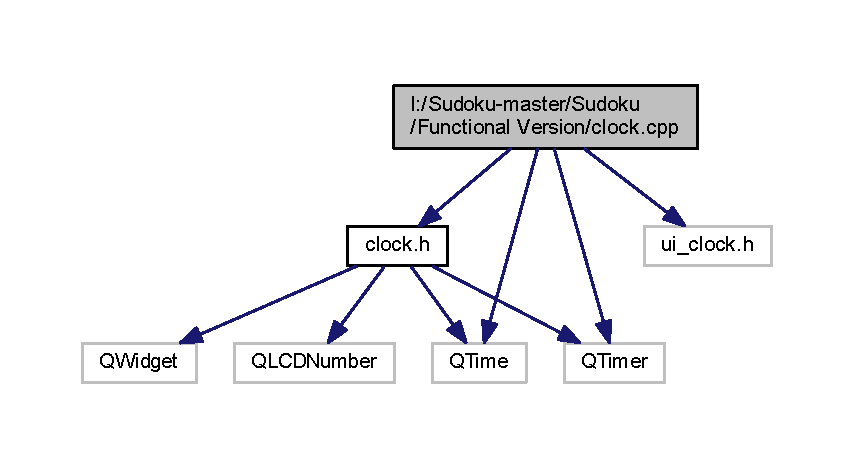
\includegraphics[width=350pt]{clock_8cpp__incl}
\end{center}
\end{figure}

\section{Referencia del Archivo I\-:/\-Sudoku-\/master/\-Sudoku/\-Functional Version/clock.h}
\label{clock_8h}\index{I\-:/\-Sudoku-\/master/\-Sudoku/\-Functional Version/clock.\-h@{I\-:/\-Sudoku-\/master/\-Sudoku/\-Functional Version/clock.\-h}}
{\ttfamily \#include $<$Q\-Widget$>$}\\*
{\ttfamily \#include $<$Q\-L\-C\-D\-Number$>$}\\*
{\ttfamily \#include $<$Q\-Time$>$}\\*
{\ttfamily \#include $<$Q\-Timer$>$}\\*
Dependencia gráfica adjunta para clock.\-h\-:
\nopagebreak
\begin{figure}[H]
\begin{center}
\leavevmode
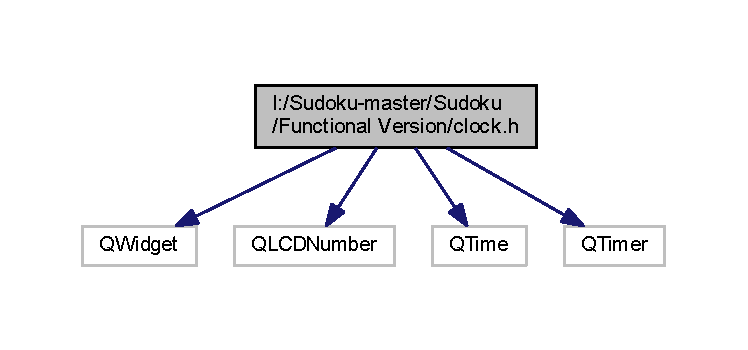
\includegraphics[width=350pt]{clock_8h__incl}
\end{center}
\end{figure}
Gráfico de los archivos que directa o indirectamente incluyen a este archivo\-:
\nopagebreak
\begin{figure}[H]
\begin{center}
\leavevmode
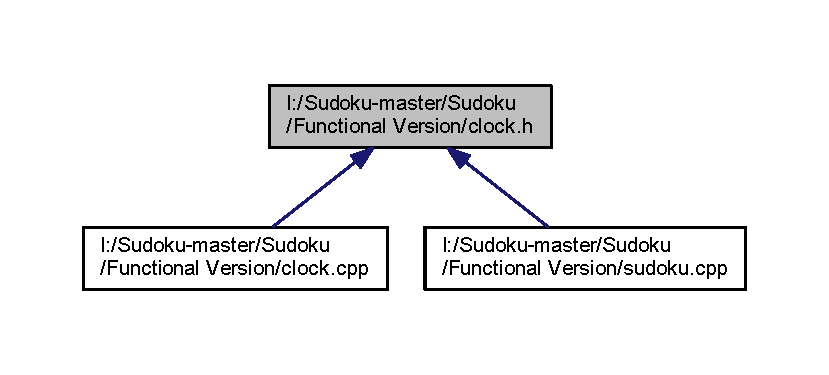
\includegraphics[width=350pt]{clock_8h__dep__incl}
\end{center}
\end{figure}
\subsection*{Clases}
\begin{DoxyCompactItemize}
\item 
class {\bf Clock}
\end{DoxyCompactItemize}
\subsection*{Namespaces}
\begin{DoxyCompactItemize}
\item 
{\bf Ui}
\end{DoxyCompactItemize}
\subsection*{Constant Groups}
\begin{DoxyCompactItemize}
\item 
{\bf Ui}
\end{DoxyCompactItemize}

\section{Referencia del Archivo I\-:/\-Sudoku-\/master/\-Sudoku/\-Functional Version/main.cpp}
\label{main_8cpp}\index{I\-:/\-Sudoku-\/master/\-Sudoku/\-Functional Version/main.\-cpp@{I\-:/\-Sudoku-\/master/\-Sudoku/\-Functional Version/main.\-cpp}}
{\ttfamily \#include \char`\"{}sudoku.\-h\char`\"{}}\\*
{\ttfamily \#include $<$Q\-Application$>$}\\*
Dependencia gráfica adjunta para main.\-cpp\-:
\nopagebreak
\begin{figure}[H]
\begin{center}
\leavevmode
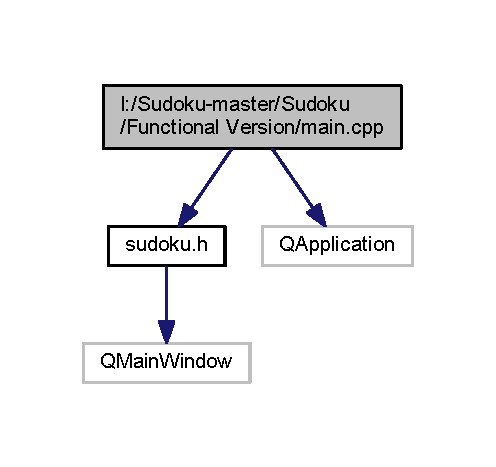
\includegraphics[width=238pt]{main_8cpp__incl}
\end{center}
\end{figure}
\subsection*{Funciones}
\begin{DoxyCompactItemize}
\item 
int {\bf main} (int argc, char $\ast$argv[$\,$])
\end{DoxyCompactItemize}


\subsection{Documentación de las funciones}
\index{main.\-cpp@{main.\-cpp}!main@{main}}
\index{main@{main}!main.cpp@{main.\-cpp}}
\subsubsection[{main}]{\setlength{\rightskip}{0pt plus 5cm}int main (
\begin{DoxyParamCaption}
\item[{int}]{argc, }
\item[{char $\ast$}]{argv[$\,$]}
\end{DoxyParamCaption}
)}\label{main_8cpp_a0ddf1224851353fc92bfbff6f499fa97}

\begin{DoxyCode}
5 \{
6     QApplication a(argc, argv);
7     Sudoku w;
8     w.show();
9     
10     \textcolor{keywordflow}{return} a.exec();
11 \}
\end{DoxyCode}

\section{Referencia del Archivo I\-:/\-Sudoku-\/master/\-Sudoku/\-Functional Version/qpushbuttongrid.cpp}
\label{qpushbuttongrid_8cpp}\index{I\-:/\-Sudoku-\/master/\-Sudoku/\-Functional Version/qpushbuttongrid.\-cpp@{I\-:/\-Sudoku-\/master/\-Sudoku/\-Functional Version/qpushbuttongrid.\-cpp}}
{\ttfamily \#include \char`\"{}qpushbuttongrid.\-h\char`\"{}}\\*
{\ttfamily \#include \char`\"{}ui\-\_\-qpushbuttongrid.\-h\char`\"{}}\\*
Dependencia gráfica adjunta para qpushbuttongrid.\-cpp\-:
\nopagebreak
\begin{figure}[H]
\begin{center}
\leavevmode
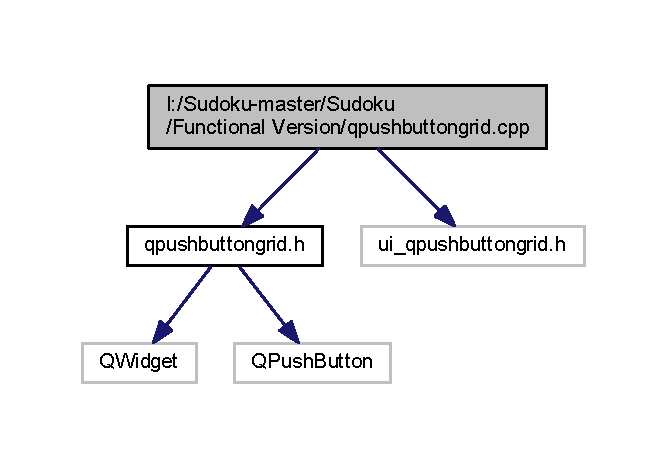
\includegraphics[width=320pt]{qpushbuttongrid_8cpp__incl}
\end{center}
\end{figure}

\section{Referencia del Archivo I\-:/\-Sudoku-\/master/\-Sudoku/\-Functional Version/qpushbuttongrid.h}
\label{qpushbuttongrid_8h}\index{I\-:/\-Sudoku-\/master/\-Sudoku/\-Functional Version/qpushbuttongrid.\-h@{I\-:/\-Sudoku-\/master/\-Sudoku/\-Functional Version/qpushbuttongrid.\-h}}
{\ttfamily \#include $<$Q\-Widget$>$}\\*
{\ttfamily \#include $<$Q\-Push\-Button$>$}\\*
Dependencia gráfica adjunta para qpushbuttongrid.\-h\-:
\nopagebreak
\begin{figure}[H]
\begin{center}
\leavevmode
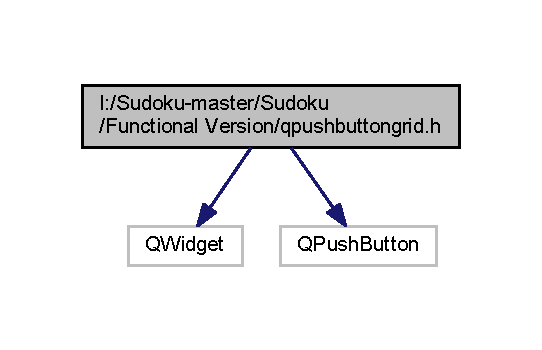
\includegraphics[width=260pt]{qpushbuttongrid_8h__incl}
\end{center}
\end{figure}
Gráfico de los archivos que directa o indirectamente incluyen a este archivo\-:
\nopagebreak
\begin{figure}[H]
\begin{center}
\leavevmode
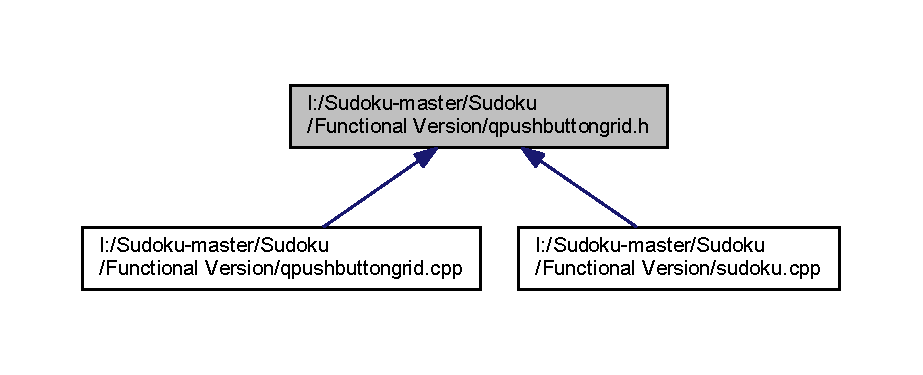
\includegraphics[width=350pt]{qpushbuttongrid_8h__dep__incl}
\end{center}
\end{figure}
\subsection*{Clases}
\begin{DoxyCompactItemize}
\item 
class {\bf Q\-Push\-Button\-Grid}
\end{DoxyCompactItemize}
\subsection*{Namespaces}
\begin{DoxyCompactItemize}
\item 
{\bf Ui}
\end{DoxyCompactItemize}
\subsection*{Constant Groups}
\begin{DoxyCompactItemize}
\item 
{\bf Ui}
\end{DoxyCompactItemize}

\section{Referencia del Archivo I\-:/\-Sudoku-\/master/\-Sudoku/\-Functional Version/sudoku.cpp}
\label{sudoku_8cpp}\index{I\-:/\-Sudoku-\/master/\-Sudoku/\-Functional Version/sudoku.\-cpp@{I\-:/\-Sudoku-\/master/\-Sudoku/\-Functional Version/sudoku.\-cpp}}
{\ttfamily \#include \char`\"{}sudoku.\-h\char`\"{}}\\*
{\ttfamily \#include \char`\"{}ui\-\_\-sudoku.\-h\char`\"{}}\\*
{\ttfamily \#include $<$Q\-Application$>$}\\*
{\ttfamily \#include $<$Q\-Push\-Button$>$}\\*
{\ttfamily \#include $<$qpushbuttongrid.\-h$>$}\\*
{\ttfamily \#include $<$Q\-Grid\-Layout$>$}\\*
{\ttfamily \#include $<$Q\-Debug$>$}\\*
{\ttfamily \#include $<$Q\-Time$>$}\\*
{\ttfamily \#include $<$Qt\-Global$>$}\\*
{\ttfamily \#include $<$math.\-h$>$}\\*
{\ttfamily \#include $<$Q\-File$>$}\\*
{\ttfamily \#include $<$Q\-Dialog$>$}\\*
{\ttfamily \#include $<$clock.\-h$>$}\\*
{\ttfamily \#include $<$stdlib.\-h$>$}\\*
{\ttfamily \#include \char`\"{}time.\-h\char`\"{}}\\*
{\ttfamily \#include $<$Q\-Reg\-Exp$>$}\\*
{\ttfamily \#include $<$Q\-File\-Dialog$>$}\\*
Dependencia gráfica adjunta para sudoku.\-cpp\-:
\nopagebreak
\begin{figure}[H]
\begin{center}
\leavevmode
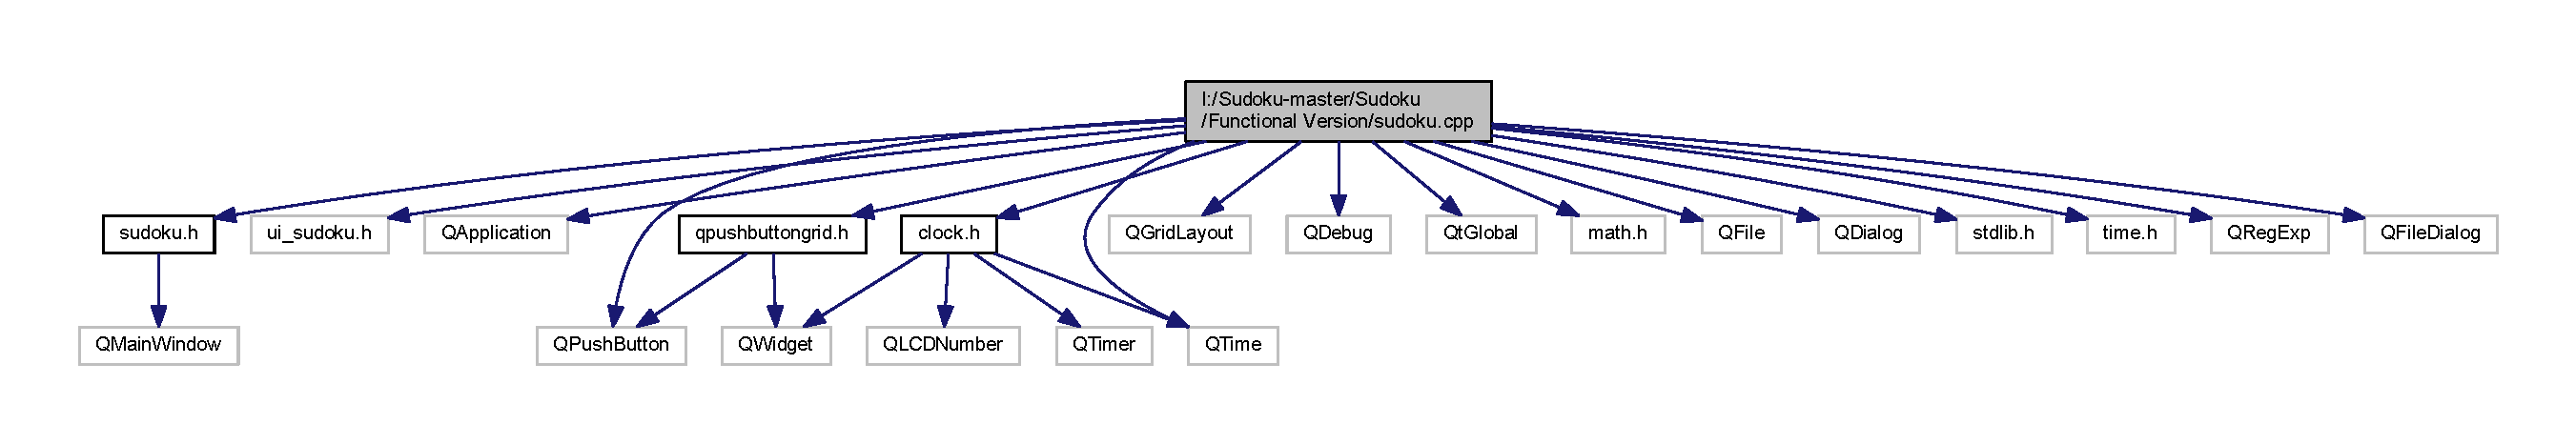
\includegraphics[width=350pt]{sudoku_8cpp__incl}
\end{center}
\end{figure}

\section{Referencia del Archivo I\-:/\-Sudoku-\/master/\-Sudoku/\-Functional Version/sudoku.h}
\label{sudoku_8h}\index{I\-:/\-Sudoku-\/master/\-Sudoku/\-Functional Version/sudoku.\-h@{I\-:/\-Sudoku-\/master/\-Sudoku/\-Functional Version/sudoku.\-h}}
{\ttfamily \#include $<$Q\-Main\-Window$>$}\\*
Dependencia gráfica adjunta para sudoku.\-h\-:
\nopagebreak
\begin{figure}[H]
\begin{center}
\leavevmode
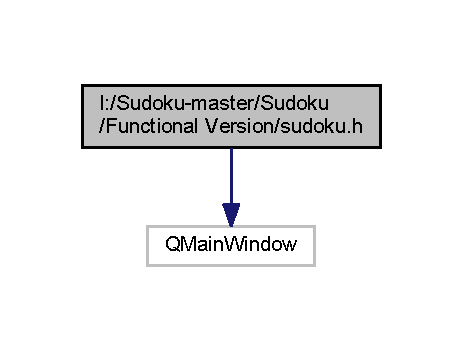
\includegraphics[width=222pt]{sudoku_8h__incl}
\end{center}
\end{figure}
Gráfico de los archivos que directa o indirectamente incluyen a este archivo\-:
\nopagebreak
\begin{figure}[H]
\begin{center}
\leavevmode
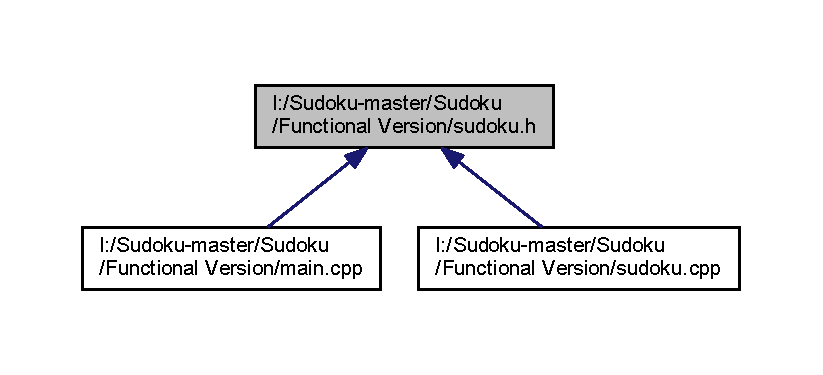
\includegraphics[width=350pt]{sudoku_8h__dep__incl}
\end{center}
\end{figure}
\subsection*{Clases}
\begin{DoxyCompactItemize}
\item 
class {\bf Sudoku}
\end{DoxyCompactItemize}
\subsection*{Namespaces}
\begin{DoxyCompactItemize}
\item 
{\bf Ui}
\end{DoxyCompactItemize}
\subsection*{Constant Groups}
\begin{DoxyCompactItemize}
\item 
{\bf Ui}
\end{DoxyCompactItemize}

%--- End generated contents ---

% Index
\newpage
\phantomsection
\addcontentsline{toc}{part}{Índice}
\printindex

\end{document}
